\documentclass[a4paper,10pt,smallheadings,twocolumn]{scrartcl}

\usepackage{times}
\usepackage[T1]{fontenc}
\usepackage[utf8]{inputenc}
\usepackage{verbatimbox}
\usepackage[autostyle=true,german=quotes]{csquotes}
\usepackage{amsmath}
\usepackage{amsfonts}
\usepackage[top=2cm,right=2cm,bottom=3cm,left=2cm]{geometry}
\usepackage{fancyhdr}
\usepackage[lastpage,user]{zref}
\usepackage{multirow}
\usepackage{mathrsfs}
\usepackage{graphicx}
\usepackage{array}
\usepackage{multirow}

\newcommand{\Title}{Computer Graphics Zusammenfassung}
\newcommand{\Author}{Lucien Zürcher}
\newcommand{\Date}{\today}

\newcommand{\norm}[1]{\lvert\lvert #1 \rvert\rvert}

\title{\vspace{-1cm}\Title\vspace{0cm}}
\date{\Date}
\author{Lucien Zürcher}

\graphicspath{ {./assets/} }


\pagestyle{fancy}
\fancyhf{}
\fancyhead[L]{\Title}
\fancyhead[R]{\Author}
\fancyfoot[L]{CG}
\fancyfoot[C]{\Date}
\fancyfoot[R]{Page \thepage\ of \zpageref{LastPage}}
\renewcommand{\headrulewidth}{0.4pt}
\renewcommand{\footrulewidth}{0.4pt}

\setlength{\columnsep}{1cm}
\setlength{\parindent}{0cm}

\newenvironment{tightenumerate}{
\begin{enumerate}
	\setlength{\itemsep}{0pt}
	\setlength{\parskip}{0pt}
}{\end{enumerate}}

\newenvironment{tighitemize}{
\begin{itemize}
	\setlength{\itemsep}{0pt}
	\setlength{\parskip}{0pt}
	\renewcommand\labelitemi{-}
}{\end{itemize}}

\begin{document}

\maketitle
\thispagestyle{fancy}
\tableofcontents
\clearpage

\section{Farbe}

\subsection{Was ist Farbe?}

\begin{itemize}
    \item \textbf{Physikalisch}, Lichtzusammensetzung, Elektromagnetischestrahlen
    \item \textbf{Physologisch}, Warnehmung und Interpretation
\end{itemize}

\textit{Farbe besteht aus:}

\begin{itemize}
    \item Farbton/Farbe
    \item Farbstich/Sättigung
    \item Helligkeit
\end{itemize}

\subsection{Farbe eines Objektes}

\textit{
    Ein Objekt nimmt Farbe auf und strahlt Farbe ab.
    Die Farbe des Objektes ist definiert durch die abgestrahlte
    Farbe.
}

\begin{itemize}
    \item Beleuchtung (Illumination)
    \item Reflektion (Reflection)
    \item Farbsignal (Color Signal)
\end{itemize}

\subsection{Licht besteht aus?}

\textit{
    Licht besitzt verschiedene Wellenlängen,
    Kombinationen dieser Frequenzen ergeben eine Farbe.
}

\begin{itemize}
    \item Sichtbares Licht (380mn - 780mn)
    \item Infrarot (780mn+)
    \item Ultraviolet (-380mn)
\end{itemize}

\textit{1nm = 10\AA (\AA ngström)} \\
\textit{1\AA = \o Atom}

\subsection{Das Auge}

\textit{
    Das Auge besteht aus; \textbf{Iris} (Muskel und Lichteinschränken),
    \textbf{Linse}, \textbf{Pupille} (Kontrolliert Iris) und \textbf{Retina}
    (Farb- und Lichtaufnahme am Rand des Auges)
} \\
\\
\textit{
    Die Retina besteht aus 75-100 $10^6$ Stäbchen (Lichtintensität) und
    6-7 $10^6$ Zäpfchen (Farbe). Die Forea ist der dichteste Platz.
}

\subsection{Wie sehen wir Farbe?}

\textit{Durch die 3 Arten von Zäpfchen:}

\begin{tabular}{ccccc}
    Kurz (S) & & Mittel (M) & & Lang (L) \\
    Blau     & & Grün       & & Rot \\
    440mn    & & 530mn      & & 560mn \\
    1        &:& 5          &:& 10 \\
\end{tabular}

\subsection{Wahrnehmung}

\textit{Grün 530mn wird am intensivsten wargenommen}

\textit{
    Die Helligkeitswahrnehmung zwischen Stäbchen und
    Zäpfchen ist unterschiedlich
}

\subsection{Farbsysteme}

\begin{itemize}
    \item \textbf{RGB} (Monitor, Spotligths,Pointilismus), \\
          additiv, C = (Rot, Grün, Blau)
    \item \textbf{CMY} (Drucken), \\
          subtraktiv, C = (Cyan, Magenta, Yellow)
    \item \textbf{CMYK}, CMY Mit Schwarz erweitert, \\
          K = min(Cyan, Magenta, Yellow) \\
          $C = C - K$, $M = M - K$, $Y = Y - K$
    \item \textbf{HSV}, \
          Farbton (Hue) / \
          Reinheit,Sättigung (Saturation) / \
          Intensität (Value)
    \item \textbf{YUV} (Alte Fernseher, UV = 1/4 Auflösung Farbkorrektur)\\
          Y = $0.229*R+0.587G+0.114*B$, \\
          U = $0.436(B-Y)/(1-0.114)$, \\
          V = $0.615(R-Y)/(1-0.299)$
    \item \textbf{CIE-Lab}, absolutes Farbsystem \\
          Achsensystem mit Helligkeit als Y-Achse und X/Z-Achse definieren Farbunterschiede
\end{itemize}

\subsection{Additives Farbsystem}

\textit{Farben additeren}
\textit{(1,1,1) = Weiss, (0,0,0) = Schwarz}

\subsection{Subtraktives Farbsystem}

\textit{Farben absorbieren}
\textit{(0,0,0) = Weiss, (1,1,1) = Schwarz}

\subsection{Farben Konvertieren}

\textit{Zu Grau: $I = 0.229*R+0.587G+0.114*B$} \\

\textit{RGB <> CMY: }
$\begin{pmatrix} C \\ M \\ Y \end{pmatrix} =
\begin{pmatrix} 1 \\ 1 \\ 1 \end{pmatrix} -
\begin{pmatrix} R \\ G \\ B \end{pmatrix}$ \\

\textit{HSV <> RGB: }\\
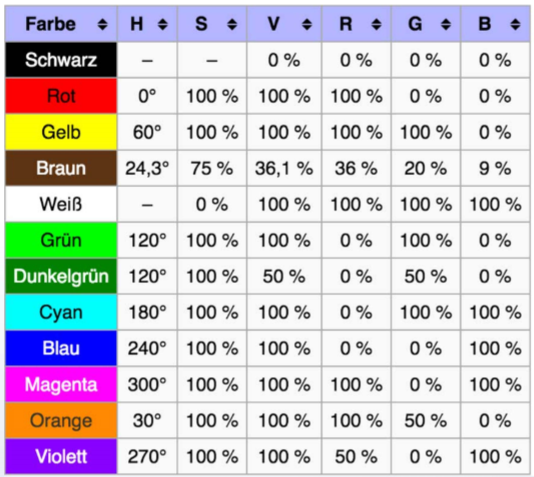
\includegraphics[width=0.4\textwidth]{assets/hsv-rgb.png}

\subsection{Gamma Korrektur}

\textit{
    Erreichen von gleichmässiger Verteilung der Helligkeit / Kontrast.
    Das Empfinden der Helligkeit ist nicht linear.
} \\
\\
\textit{
    Korrektur der Helligkeit des Bildes mit Gamme Wert. Wichtig für Bildschirme einstellen.
    Beim einstellen der Monitore Grauwerte mit echten Werten vergleichen (Gamma Test Pattern).
}

\subsection{Normfarbtafel}

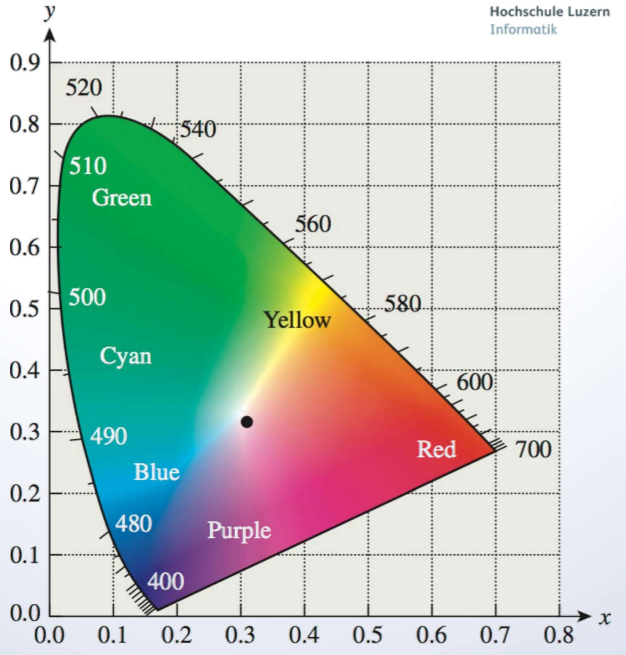
\includegraphics[width=0.4\textwidth]{assets/color-cie.png}

\subsection{Helligkeitswahrnehmung}

\textit{Helligkeit wird logarithmisch wahrgenommen, Webers Law}

$\frac{\Delta I}{I} = C$ \\
$\log (I + \Delta I) - \log(I) = Const$

\subsection{Nibs (Lichtdichte)}

\textit{
    Gibt Helligkeitsdichte für Auge an. 10nits werden stärker wargenommen denn 100nits.
    Heisst, weniger Licht wird stärker wargenommen.
}

\subsection{Mach bending}

\textit{
    Optische Illusion, bei zwei verschiedenen Grauwerten nebeneinander
    unterschieden sich diese vermeitlich stärker.
}

\subsection{Farbtäschung}

\textit{
    Farbe wird abhängig durch Umgebung anderst wargenommen
    (Dunkler, Heller). Optische Illusionen
}

\subsection{HD,UHD,UK}

\textit{Unterscheiden sich durch Pixelauflösung.}

\subsection{Was ist HDR?}

\textit{
    \textbf{High Dynamic Range}, speichert zusätzlichen Wert um
    Helligkeitsunterschiede besser unterschieden zu können
    (RGB-Pixelwerte propertianal zum Licht).
    Detailreichere dunkel und helle Spots, weniger Verlust
    durch Farben mit weniger Helligkeitsunterschiede.
}

\subsection{Begriffe}

\begin{tabular}{r|l}
    \textbf{Natürliches Licht}  & Gemisch aus verschiedenen \\
                                & Lichtwellen / Frequenzen \\
    \textbf{Spektralfarben}     & reine Farbfrequenz; Alle Farben \\
                                & am Rand des CIE-Farbsystems \\
    \textbf{Spektrum}           & Alle Frequenzen und deren \\
                                & Verteilung \\
    \textbf{Spektralverteilung} & Charakterisiert die Farbe, definiert \\
                                & durch Frequenzen \\
                                & (Bsp. Verschiedenes Weiss) \\
    \textbf{Komplementärfarben} & Addieren ergeben Grau, \\
                                & gegenüberligende Farben im \\
                                & CIE-Farbsystem
\end{tabular}

\section{Halbtontechnik}


\section{WebGL}

\subsection{OpenGL Merkmale}

\begin{itemize} \setlength\itemsep{0em}
    \item Low Level Graphics API
    \item Verschiedene Platformen
    \item 1.0/2.0 Fixe Funktionspipeline
    \item Vorlage für WebGL
\end{itemize}

\subsection{Grafikpipeline}

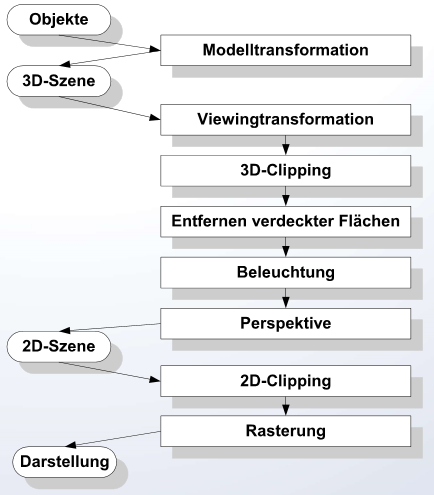
\includegraphics[width=0.4\textwidth]{assets/grafikpipline.png}

\subsection{Programmierbare Shaders}

\textit{
    Shaders werden für die Berechnung der zu zeichnenden
    Objekte verwendet. Das Programm wird direkt auf der Grafikkarte
    ausgeführt.
}

\subsubsection{Vertex Processing / Vertex Shader}

\textit{
    Berechnen der \textbf{Positionen} der Vertexe (Punkte) und
    Werte für den folgenden Fragmentshader.
}

\subsubsection{Fragment Processing / Fragment Shader}

\textit{
    Berechnet die \textbf{Farbe} der einzelnen Pixel.
}

\subsection{Datenfluss}

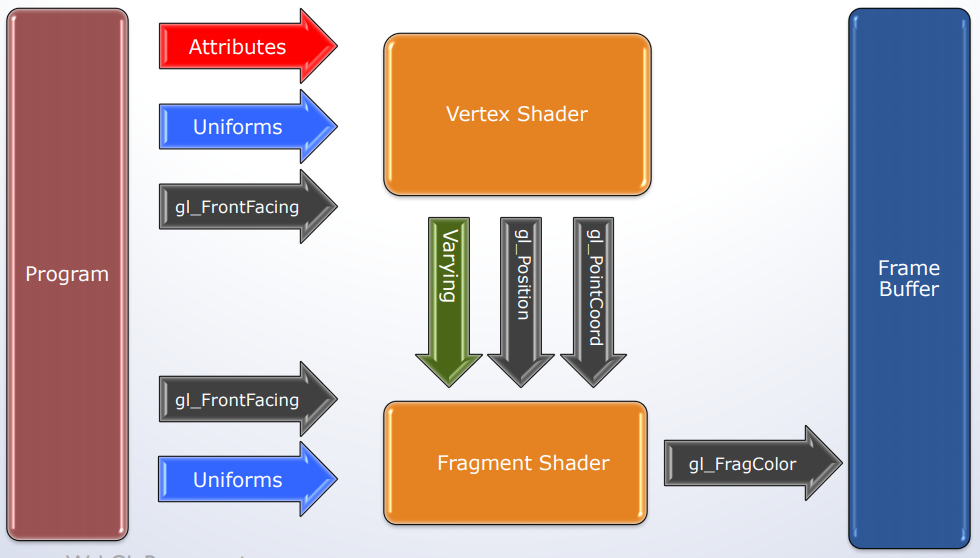
\includegraphics[width=0.5\textwidth]{assets/dataprocessing.png}

\subsection{Attribute und Uniform Variablen mit Shaders verbinden}

\begin{enumerate}
	\item Attribute \\
	\texttt{ctx.aVertexPositionId = gl.getAttribLocation(ctx.shaderProgram, "aVertexPosition")}
	
	\item Uniform \\
	\texttt{ctx.uColorId = gl.getUniformLocation(ctx.shaderProgram, "uColor"))}
	
\end{enumerate}

\subsection{Attribut Variablen und Buffer definieren}

\textbf{Erzeugen}

\begin{enumerate}
    \item Buffer erzeugen \\
    \texttt{var buffer = gl.createBuffer()}
    
    \item Array Buffer auf Buffer setzen \\
    \texttt{gl.bindBuffer(gl.ARRAY\_BUFFER, buffer)}
    
    \item Daten füllen \\
    \texttt{gl.BufferData(gl.ARRAY\_BUFFER, new Float32Array(vertices), gl.STATIC\_DRAW)}
\end{enumerate}

\textbf{Zeichnen}

\begin{enumerate}
    \item Buffer binden
    \item Attribut und/oder uniform setzen \\
    \texttt{gl.vertexAttribPointer(index, size, type, normalized, stride, offset)} \\
    z.B. \texttt{gl.vertexAttribPointer(ctx.aVertexPositionId, 2, gl.FLOAT, false, 0, 0)}
    
    \item Attribut als Array setzen \\
    \texttt{gl.enableVertexAttribArray(index)}
    
    \item Zeichnen \\
    \texttt{gl.drawArrays(mode, first, count)}
\end{enumerate}

\newpage

\section{Vektoren}

\textit{$\bullet$ Skalarprodukt} \\
\textit{$\cdot$ Matrixprodukt} \\
\textit{$\times$ Kreuzprodukt}

\subsection{Addition}

$\vec{a} + \vec{b} = \begin{bmatrix}
    a_1 \\
    a_2 \\
    a_n \\
\end{bmatrix} + \begin{bmatrix}
    b_1 \\
    b_2 \\
    b_n \\
\end{bmatrix} = \begin{bmatrix}
    a_1 + b_1 \\
    a_2 + b_2 \\
    a_n + b_n \\
\end{bmatrix}$

\subsection{Multiplikation mit Skalar}

$\lambda \vec{a} = \lambda\begin{bmatrix}
    a_1 \\
    a_2 \\
    a_n \\
\end{bmatrix} = \begin{bmatrix}
    \lambda a_1 \\
    \lambda a_2 \\
    \lambda a_n \\
\end{bmatrix}$ \\

\textit{$\lambda \in$ Skalar}

\subsection{Nullvektor}

$\vec{0} = \begin{bmatrix}
    0 \\
    0 \\
\end{bmatrix}$

\subsection{Vektorinverses}

$-\vec{a} = - \begin{bmatrix}
    a_1 \\
    a_2 \\
    a_n \\
\end{bmatrix} = \begin{bmatrix}
    -a_1 \\
    -a_2 \\
    -a_n \\
\end{bmatrix}$

\textit{Vektor mit negativen Komponenten}

\subsection{Vektoren Gleichheit}

$\vec{a} = \begin{bmatrix}
    3 \\
    2
\end{bmatrix} = \vec{b}$

\textit{Vektoren sind gleich, wenn Komponenten gleich}

\subsection{Skalarprodukt}

$\vec{a} \bullet \vec{b} = \begin{bmatrix}
    a_1 \\
    a_2 \\
    a_n
\end{bmatrix} \bullet \begin{bmatrix}
    b_1 \\
    b_2 \\
    b_n
\end{bmatrix} = a_1 b_1 + a_2 b_2 + \dots + a_n b_n$

\begin{tabular}{cc}
    \multirow{6}{*}{
        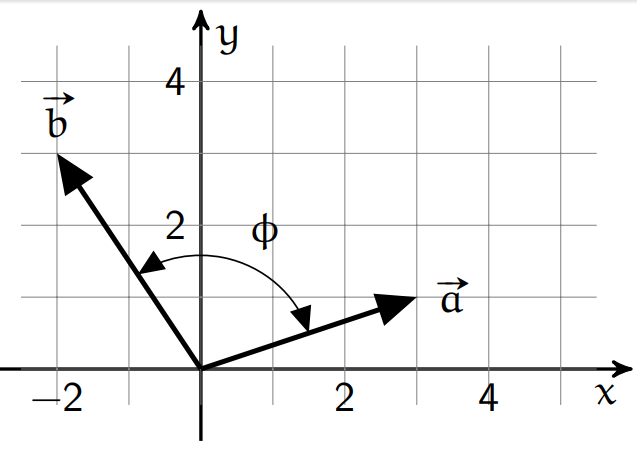
\includegraphics[width=0.25\textwidth]{assets/skaparprodukt.png}
    }
     & $\vec{a} \bullet \vec{b} = |\vec{a}| \cdot |\vec{b}| \cdot \cos \phi$ \\
     & \\
     & $|\vec{a}| = \sqrt{a_1^2 + a_2^2 + \dots + a_n^2}$ \\
     & $|\vec{b}| = \sqrt{b_1^2 + b_2^2 + \dots + b_n^2}$ \\
     & \\
     & $\cos \phi = \frac{\vec{a} \bullet \vec{b}}{|\vec{a}| \cdot |\vec{b}|}$ \\
\end{tabular}

\subsection{Skalarprodukt im beliebigem Koordinatensystem}

$\vec{a} = a_1\vec{e}_1 + a_2\vec{e}_2 + a_3\vec{e}_3 = [a_1 a_2 a_3]^T$ \\
$\vec{b} = b_1\vec{e}_1 + b_2\vec{e}_2 + b_3\vec{e}_3 = [b_1 b_2 b_3]^T$ \\

$\vec{a} \bullet \vec{b} = [a_1 a_2 a_3]\begin{bmatrix}
    g_{11} & g_{12} & g_{13} \\
    g_{21} & g_{22} & g_{23} \\
    g_{31} & g_{32} & g_{33} \\
\end{bmatrix} \begin{bmatrix}
    b_1 \\
    b_2 \\
    b_3
\end{bmatrix} = \mathbf{a}^T \mathbf{G} \mathbf{b}$

\textit{Matrix $\mathbf{G}$ wird \textbf{metrisch Tensor} genannt}

\subsection{Orthogonal}

$\vec{e}_x \bullet \vec{e}_y = 0$ \\
$\vec{a} \bullet \vec{b} = 0 \Leftrightarrow \vec{a} \bot \vec{b}$

\textit{
    Senkrecht zueinander, wenn Skalarprodukt zweier Einheitsvektoren 0 ergibt.
}

\subsection{Länge des Vektors}

$|\vec{a}| = \sqrt{\vec{a} \bullet \vec{a}} = \sqrt{a_1^2 + a_2^2 + \dots + a_n^2}$

\subsection{Einheitsvektor}

$ e_v = \frac{1}{\norm{v}} \bullet v = \frac{1}{\sqrt{v \cdot v}} \bullet v$ \\
$ ( i = e_1, j = e_2, k = e_3 ) $ \\

\textit{$\vec{e}_x = [1,0,0]^T$}\\
\textit{$\vec{e}_y = [0,1,0]^T$}\\
\textit{$\vec{e}_z = [0,0,1]^T$}

\subsection{Euklidische Distanz}

$\bar{AB} = \sqrt{(b_1-a_1)^2 + (b_2 - a_2)^2 + \dots + (b_n - a_n)^2}$

\subsection{Gerade im 2/3D}

\begin{itemize}
    \item \textbf{Punkt-Punktform mit Vektoren 2/3D} \\
          $\vec{r} = \vec{r}_1 + t(\vec{r}_2 - \vec{r}_1)$, $t \in \mathbb{R}$ \\
          $\vec{r}_1$: Punkt, $\vec{r}_2$: Punkt
    \item \textbf{Punkt-Richtungsform mit Vektoren 2/3D} \\
          $\vec{r} = \vec{r}_0 + t\vec{r}_1$, $t \in \mathbb{R}$ \\
          $\vec{r}_0$: Punkt, $\vec{r}_1$: Richtungsvektor
    \item \textbf{Achsenabschnitt-Steigungsform} \\
          $y=mx+b$ \\
          $b$: Achsenabschnitt, $m$: Steigung
    \item \textbf{Punkt-Richtungsform} \\
          $(y - y_0) = m(x - x_0)$ \\
          ($x_0$,$y_0$): Punkt, $m$: Steigung
    \item \textbf{Allgemeine Geradengleichung} \\
          $ax + by + c = 0$ \\
          $a,b,c \in \mathbb{R}$\\
    	  \\
    	  Aus Punkten A(x1, y1) und B(x2, y2) \\
    	  $\frac{y2 - y1}{x2 - x1} = \frac{y - y1}{x - x1}$
\end{itemize}

\subsection{Hessische Normalform}

\textit{Viktorielle Schreibweise der Hessischen Normalform}
\begin{tabular}{cl}
    \multirow{10}{*}{
        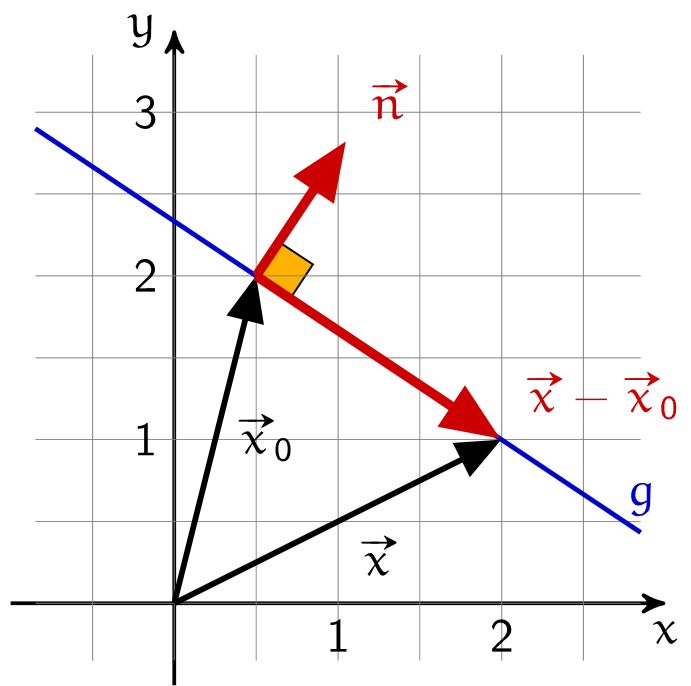
\includegraphics[width=0.2\textwidth]{assets/hessischenormalform.png}
    }
     & $\vec{n} \bullet (\vec{x} - \vec{x}_0) = 0$ \\
     & da $\vec{n} \bot (\vec{x} - \vec{x}_0)$ \\
     & $\Rightarrow n_x(x - x_0) + n_y(y - y_0) = $\\
     & $n_x x + n_y y - (n_x x_0 + n_y y_0)$\\
     & \\
     & Abstand vom Uhrsprung: $d$ \\
     & $d = (n_x x_0 + n_y y_0) = \vec{n} \bullet \vec{x}_0$\\
     & \\
     & \textit{$\vec{n}$ muss normalisiert sein:} \\
     & $|\vec{n}| = 1 \Rightarrow \frac{1}{\sqrt{n_x^2 + n_y^2}} \bullet \vec{n}$ \\
\end{tabular} \\

\begin{tabular}{cl}
    \multirow{10}{*}{
        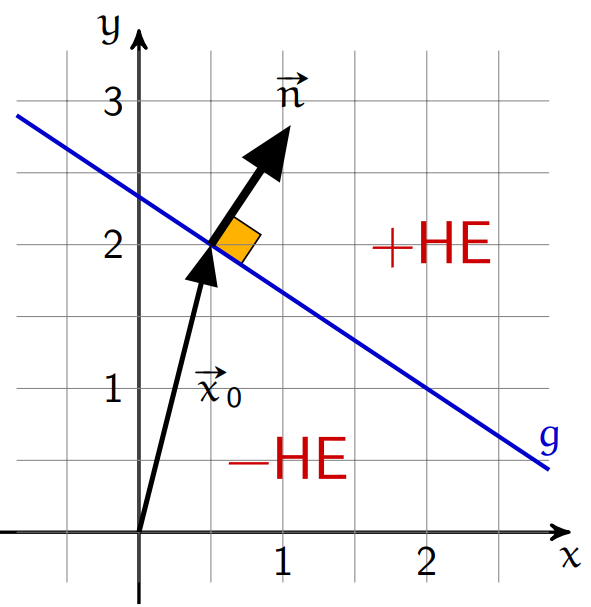
\includegraphics[width=0.2\textwidth]{assets/hessischenormalfromebene.png}
    }
     & $\mathbf{n_x x + n_y y - d = 0}$ \\
     & $d = (n_x x_0 + n_y y_0) = \vec{n} \bullet \vec{x}_0$\\
     & \\
     & $d > 0 \Leftrightarrow (0,0) \in -HE $ \\
     & $d < 0 \Leftrightarrow (0,0) \in +HE $ \\
     & \\
     & $g$: $ax + by + c = 0$\\
     & $\vec{n} = \begin{bmatrix}
         n_x \\
         n_y \\
     \end{bmatrix} = \frac{1}{\sqrt{a^2 + b^2}} \begin{bmatrix}
         a \\
         b \\
     \end{bmatrix}$ \\
     & $d = - \frac{c}{\sqrt{a^2 + b^2}}$ \\
     & \\
\end{tabular}

\textbf{Abstand eines Punktes zur Geraden berechnen}

\textit{Punkt P(x,y) einsetzten $\frac{a x + b y - d = 0}{\sqrt{a^2 + b^2}} = Abstand$}

\subsection{Hessische Normalform Ebene}

$\epsilon: ax + by + cz + d = 0$ \\

$n_x x + n_y y + n_z z - D = 0$;
\textit{HNF der Ebene $\epsilon \in \mathbb{R}^3$}

$\vec{n} = \begin{bmatrix}
    n_x \\
    n_y \\
    n_z
\end{bmatrix} = \frac{1}{\sqrt{a^2 + b^2 + c^2}} \begin{bmatrix}
    a \\
    b \\
    c
\end{bmatrix} $ \\
$D = - \frac{d}{\sqrt{a^2 + b^2 + c^2}}$

\subsection{Achsenabschnitt}

\begin{tabular}{cl}
    \multirow{5}{*}{
        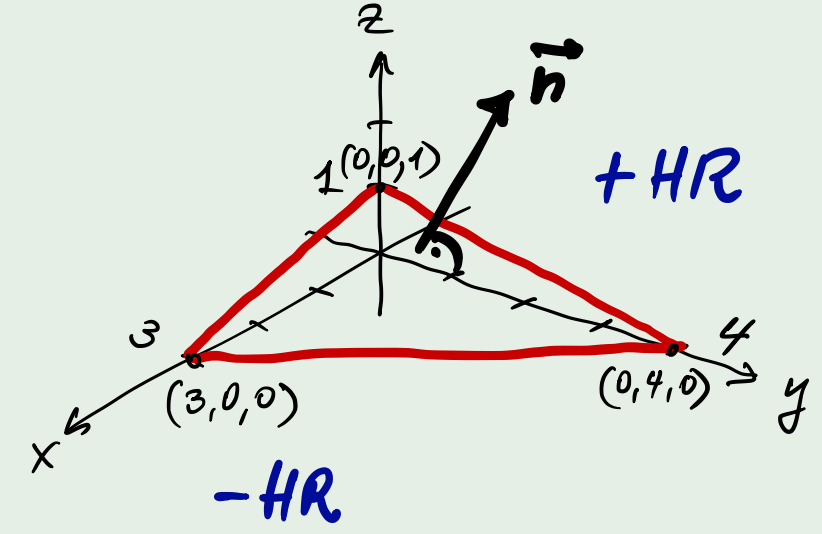
\includegraphics[width=0.2\textwidth]{assets/hnfachsenabschnitt.png}
    }
    & \textit{Gegeben sind 3 Punkte $p_x = x$, } \\
    & \textit{$p_y = y$, $p_z = z$ die ergeben eine } \\
    & \textit{Ebenegleichung:} \\
    & \\
    & $\mathbf{\frac{x}{p_x} + \frac{y}{p_y} + \frac{z}{p_z} - 1 = 0}$ \\
\end{tabular}

\subsection{Projektion eines Vektors}

\begin{tabular}{cl}
    \multirow{7}{*}{
        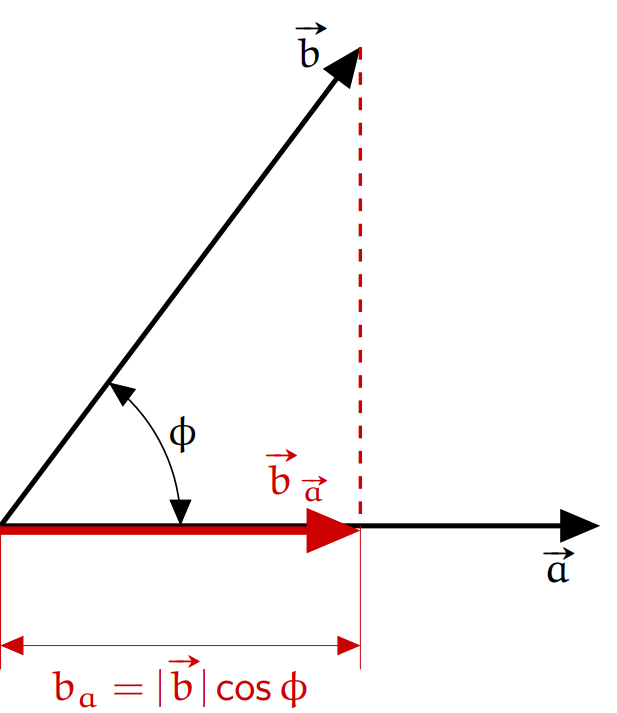
\includegraphics[width=0.15\textwidth]{assets/projection-of-vector.png}
    }
    & $\vec{b}$ Richtung $\vec{a}$:\\
    & $\vec{b}_{\vec{a}} = \frac{\vec{a} \bullet \vec{b}}{|\vec{a}|^2} \vec{a}$\\
    & \\
    & \textit{$b_a$ mal Einheitsvektor $\vec{a}$} \\
    &
        $\vec{b}_{\vec{a}} = b_a \frac{1}{|\vec{a}|} \vec{a} =
        |\vec{a}||\vec{b}|\cos \phi \frac{1}{|\vec{a}|} \vec{a}$ \\
    & $= \frac{\vec{a} \bullet \vec{b}}{|\vec{a}|^2} \vec{a}$\\
    & \\
\end{tabular}

\subsection{Vektorprodukt / Kreuzprodukt}

\begin{tabular}{cl}
    \multirow{7}{*}{
        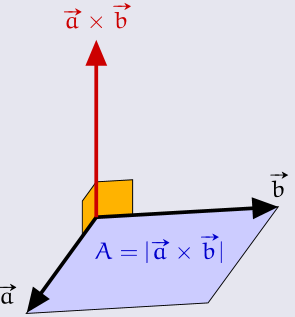
\includegraphics[width=0.15\textwidth]{assets/vectorproduct.png}
    }
    & $\vec{a} \times \vec{b}$ steht senkrecht auf beiden Vektoren \\
    & \\
    & $\vec{a}$, $\vec{b}$ und $\vec{a} \times \vec{b}$ sind ein Rechstsystem \\
    & \\
    & $\vec{a} \times \vec{b}$ entspricht der Fläche des \\
    & aufgespannten Parallelogramms ($A$): \\
\end{tabular} \\

$A = \sqrt{(a_2 b_3 - a_3 b_2)^2 + (a_3 b_1 - a_1 b_3)^2 + (a_1 b_2 - a_2 b_1)^2}$ \\

\begin{tabular}{cl}
    \multirow{5}{*}{
        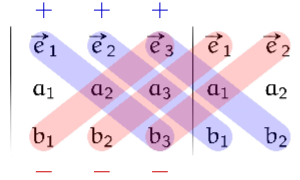
\includegraphics[width=0.15\textwidth]{assets/vectorproduct-build.png}
    }
    & $\vec{a} \times \vec{b} = \begin{bmatrix}
    		a_1 \\
    		a_2 \\
    		a_3 \\
    	\end{bmatrix} \times \begin{bmatrix}
    		b_1 \\
    		b_2 \\
    		b_3 \\
    	\end{bmatrix} = \begin{bmatrix}
    		a_2 b_3 - a_3 b_2 \\
    		a_3 b_1 - a_1 b_3 \\
    		a_1 b_2 - a_2 b_1 \\
    	\end{bmatrix}$ \\
    	& $= \begin{bmatrix}
            \vec{e}_1 & \vec{e}_2 & \vec{e}_3 \\
            a_1 & a_2 & a_3 \\
            b_1 & b_2 & b_3 \\
        \end{bmatrix}$ \\
    & $= (a_2 b_3 - a_3 b_2) \vec{e}_1 +$ \\
    & $(a_3 b_1 - a_1 b_3) \vec{e}_2 + (a_1 b_2 - a_2 b_1) \vec{e}_3 $ \\
\end{tabular} \\
\textit{Regel von Sarrus} \\

\subsection{Vektorprodukt Anwendung}

\begin{itemize}
    \item \textbf{Lorentz-Karft} $\vec{F} = q(\vec{v} \times \vec{B})$ \\
          $\vec{v}$: Geschwindigkeit, $B$: Magnetfeld, $q$: Landung
    \item \textbf{Geschwindigkeit} $\vec{v} = q(\vec{w} \times \vec{x})$ \\
          $\vec{x}$: Punkt, $w$: Winkelgeschwindigkeit, $\vec{w}$: Drehachse
    \item \textbf{Drehmoment} $\vec{M} = \vec{r} \times \vec{F}$ \\
          $\vec{F}$: Kraft, $\vec{r}$: Punkt / Koordinatenursprung
    \item \textbf{Normalvektor} $\vec{n} = \vec{a} \times \vec{b}$ \\
          $\vec{a}$ und $\vec{b}$ liegen auf der Ebene.
    \item \textbf{Kollinearität} kollinear (d.h. linear abhängig) wenn Vektorprodukt verschwinded
\end{itemize}

\subsection{Matrixprodukt}

\textit{falksche Schema} \\

$\vec{a} \cdot \vec{b} = \begin{bmatrix}
a_1 & a_3\\
a_2 & a_4\\
\end{bmatrix} \cdot \begin{bmatrix}
b_1 & b_3 \\
b_2 & b_4 \\
\end{bmatrix} = \begin{bmatrix}
a_1 b_1 + a_3 b_2 & a_1 b_3 + a_3 b_4\\
a_2 b_1 + a_4 b_2 & a_2 b_3 + a_4 b_4\\

\end{bmatrix}$ \\

\textit{In Worten für die erste Zeile: $a_1$ mal die erste Zeile + $a_3$ mal die zweite Zeile etc.. Wobei die Spalten unabhängig bleiben.}

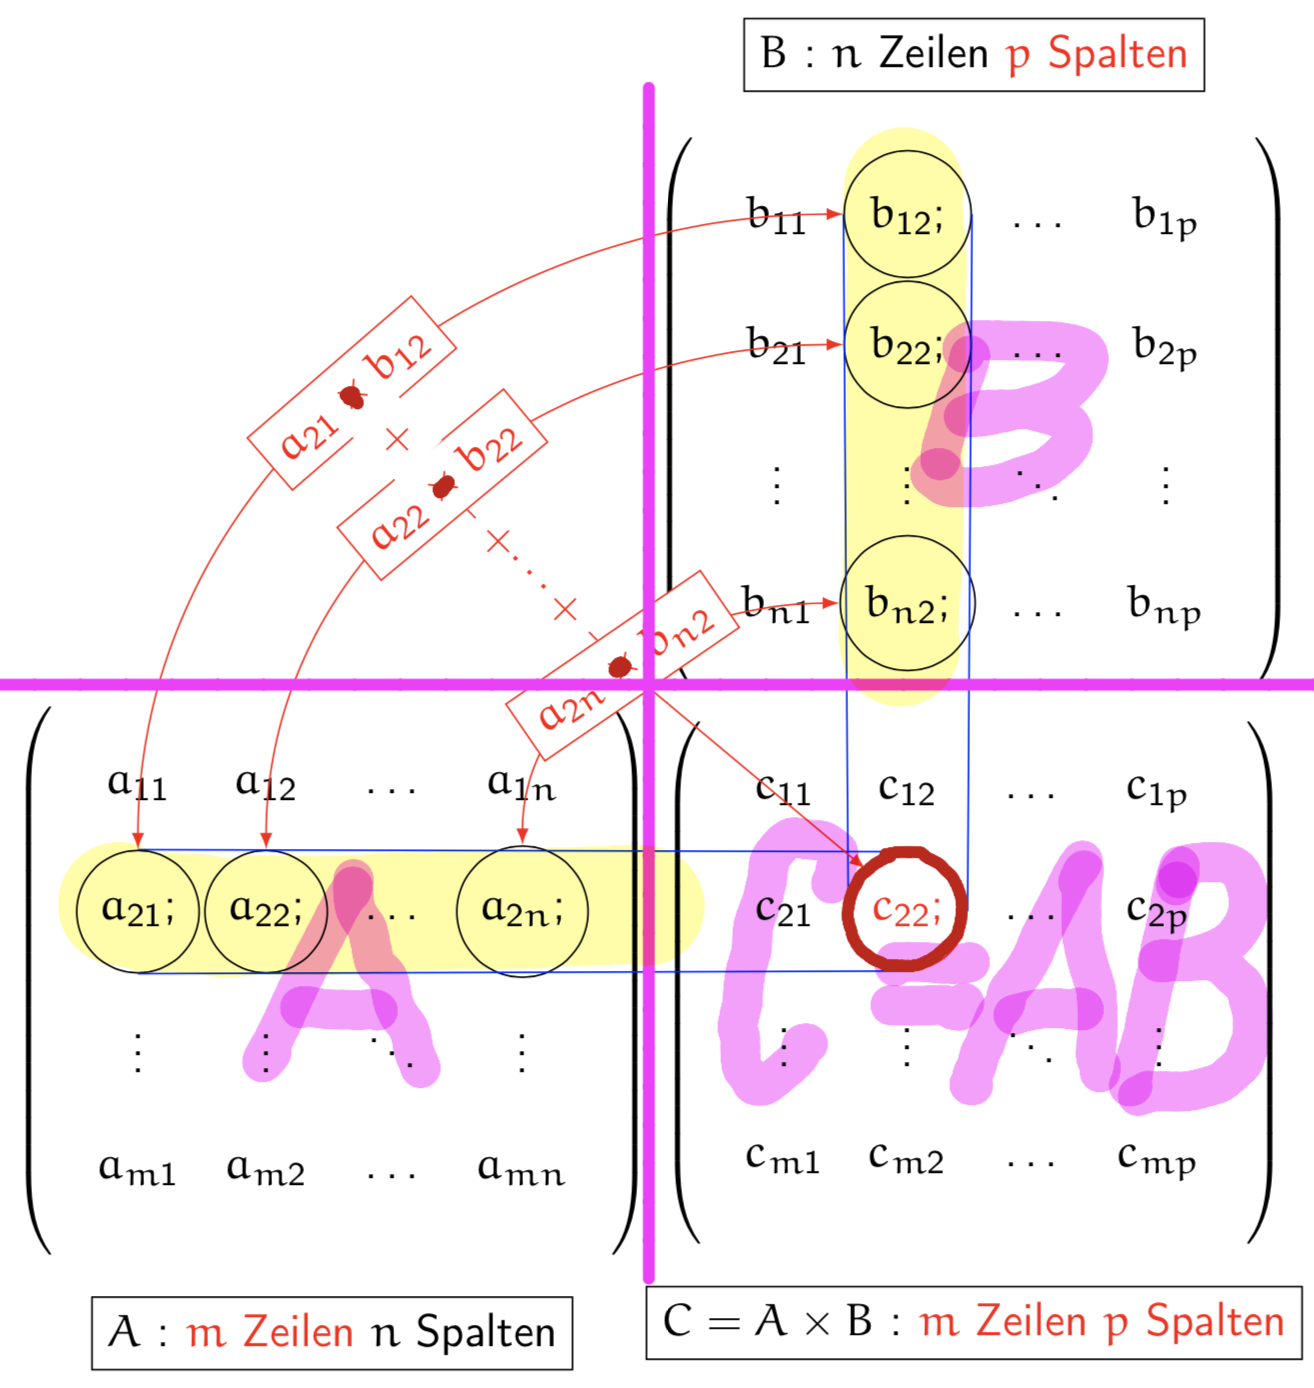
\includegraphics[width=0.45\textwidth]{assets/FalkschesSchema.png}

\subsection{Spatprodukt}

\begin{tabular}{cl}
    \multirow{6}{*}{
        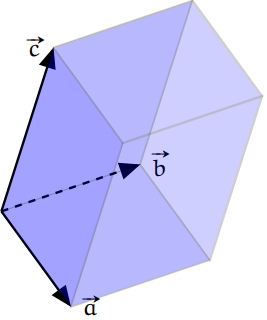
\includegraphics[width=0.12\textwidth]{assets/spatproduct.png}
    }
    & \textbf{Spatprodukt} $[\vec{a}, \vec{b}, \vec{c}]$ \\
    & \textit{Ist der Skalar der Vektoren $\vec{a}$, $\vec{b}$, $\vec{c}$} \\
    & \\
    & $[\vec{a}, \vec{b}, \vec{c}] = \vec{a} \bullet (\vec{b} \times \vec{c})$\\
    & \textit{Spatprodukt entsprich Volumen wenn in} \\
    & \textit{einem Rechstsystem, dann: $V_{Spat} = |[\vec{a}, \vec{b}, \vec{c}]|$} \\
\end{tabular} \\

$|[\vec{a}, \vec{b}, \vec{c}]| = $ \\
$a_1 b_2 c_3 + a_2 b_3 c_1 + a_3 b_1 c_2 - a_3 b_2 c_1 - a_1 b_3 c_2 - a_2 b_1 c_3$
\textit{Komplanar (linear abhängig) wenn $[\vec{a}, \vec{b}, \vec{c}] = 0$}

\subsection{Translation 2D}

$\vec{x}' = \vec{x} + \vec{t} = \begin{bmatrix}
    x_1 \\
    x_2 \\
\end{bmatrix} + \begin{bmatrix}
    t_1 \\
    t_2 \\
\end{bmatrix} = \begin{bmatrix}
    x_1 + t_1 \\
    x_2 + t_2 \\
\end{bmatrix}$

\subsection{Skalierung 2D}

$\vec{x}' = \begin{bmatrix}
    \vec{s}_x x \\
    \vec{s}_y y \\
\end{bmatrix} = \begin{bmatrix}
    s_x & 0 \\
    0 & s_y \\
\end{bmatrix} \begin{bmatrix}
    x \\
    y \\
\end{bmatrix}$

\subsection{Rotation 2D}

$\vec{x}' = \begin{bmatrix}
    x' \\
    y' \\
\end{bmatrix} = \begin{bmatrix}
    \cos(\phi) & -\sin(\phi) \\
    \sin(\phi) & \cos(\phi) \\
\end{bmatrix} \begin{bmatrix}
    x \\
    y \\
\end{bmatrix} = \mathbf{R}\vec{x}$

\textit{Inverse Matrix: $\mathbf{R}^{-1} = \mathbf{R}^T$}

\subsection{Vektor Rechenregeln}

\begin{tabular}{r|l}
    $\vec{a} + \vec{b} = \vec{b} + \vec{a}$ & Kommutativgesetz \\
    $\vec{a} + (\vec{b} + \vec{c}) = (\vec{a} + \vec{b}) + \vec{c}$ & Assoziativgesetz \\
    $\vec{a} + \vec{0} = \vec{a}$ & Existenz Neutralelement $\vec{0}$ \\
    $\vec{a} + (-\vec{a}) = \vec{0}$ & Existenz Inverses -$\vec{a}$ \\
    $\lambda(\vec{a} + \vec{b}) = \lambda \vec{a} + \lambda \vec{b}$ \\
    $(\lambda + \mu) \vec{a} = \lambda \vec{a} + \mu \vec{a}$ \\
    $(\lambda \mu) \vec{a} = \lambda(\mu \vec{a}) = \mu (\lambda \vec{a})$ \\
    $1 \vec{a} = \begin{bmatrix}
        1 \\
        1
    \end{bmatrix} \vec{a} = \vec{a}$

\end{tabular}

\subsection{Rechenregel Skalarprodukt}

$\vec{a} \bullet \vec{b} = \vec{b} \bullet \vec{a}$ \\
$\vec{a} \bullet (\vec{b} + \vec{c}) = \vec{a} \bullet \vec{b} + \vec{a} \bullet \vec{c}$ \\
$\lambda (\vec{a} \bullet \vec{b}) = (\lambda \vec{a}) \bullet \vec{b} = \vec{a} \bullet (\lambda \vec{b})$

\subsection{Vektorprodukt Rechenregeln}

\begin{tabular}{r|l}
    $\vec{a} \times \vec{b} = -\vec{b} \times \vec{a}$ & Anti-Kommutativgesetz \\
    $\vec{a} \times (\vec{b} + \vec{c}) = \vec{a} \times \vec{b} + \vec{a} \times \vec{c}$ & Distributivgesetz \\
    $\lambda (\vec{a} \times \vec{b}) = (\lambda \vec{a}) \times \vec{b} = \vec{a} \times (\lambda \vec{b})$
\end{tabular}

\subsection{Spatprodukt Rechenregeln}

\begin{tabular}{r|l}
    $[\vec{a}, \vec{b}, \vec{c}] = -[\vec{b}, \vec{a}, \vec{c}]$ & zwei Vekoren vertauschen \\
                                                                 & entspricht Vorzeichenwechsel \\
    $[\vec{a}, \vec{b}, \vec{c}] = [\vec{c}, \vec{a}, \vec{b}] $ & Zyklisches Vertauschen \\
                                                                 & keine Änderung \\
    $[\lambda \vec{a}, \mu \vec{b}, \nu \vec{c}] = \lambda\mu\nu[\vec{a}, \vec{b}, \vec{c}]$ & Multiplikation \\
    $[\vec{a} + \vec{b}, \vec{c}, \vec{d}] = $ & Addition \\
    $[\vec{a}, \vec{c}, \vec{d}] + [\vec{b}, \vec{c}, \vec{d}]$ & \\
\end{tabular}

\subsection{Begriffe}

\begin{tabular}{r|l}
    \textbf{Ortsvektor}         & Vom Ursprung zum Punkt \\
    \textbf{Richtungsvektor}    & Eine Richtung im Raum \\
    \textbf{Einheitsvektor}     & Eine Einheit in eine beliebige \\
                                & Richtung \\
    \textbf{Linearkombination}  & Ein Vektor, der ein vielfaches \\
    \textit{kollinear}          & eines Einheitvektors ist. \\
                                & $\vec{c} = \lambda\vec{a} + \mu \vec{b}$ \\
    \textbf{Linear Unabhängig}  & Vektoren sind unabhängig wenn \\
    \textit{komplanar}         & $\lambda_1 \vec{a}_1 + \lambda_2 \vec{a}_2 + \dots + \lambda_n \vec{a}_n = \vec{0}$ \\
                                & $\Leftrightarrow \lambda_1 = \lambda_2 = \dots = \lambda_n = 0$ \\
    \textbf{Skalar}             & Ist ein reelle oder komplexe Zahl \\
    \textbf{Rechtssystem}       & Koordinatensystem aufgebaut wie die \\
                                & rechte Hand wobei; der Zeigfinger \\
                                & X-Achse ($\vec{e}_x$), Mittelfinger \\
                                & Y-Achse ($\vec{e}_y$) und Daumen \\
                                & Z-Achse ($\vec{e}_z$) \\
\end{tabular}
\section{Projektive Geometrie}

\subsection{Homogener Vektor}

$\vec{r} = \begin{bmatrix}
    x_1 \\
    x_2 \\
    x_3 \\
\end{bmatrix}$
\textit{Homogener 2D Vektor} \\

$(x,y) = (\frac{x_1}{x_3}, \frac{x_2}{x_3})$

\subsection{Punkt auf Gerade}

$ax + by + c = 0 \Leftrightarrow \vec{g} \bullet \vec{r} = 0$

$\vec{r} = \begin{bmatrix}
    x \\ y \\ 1
\end{bmatrix}$,
$\vec{g} = \begin{bmatrix}
    a \\ b \\ c
\end{bmatrix}$

\textit{$A(x,y)$ (homogenisiert $\vec{r}$) liegt dann auf gerade $\vec{g}$}

\subsection{Schnittpunkt Geraden}

$\vec{r} = \vec{g}_1 \times \vec{g}_2$

$\vec{g}_1 = \begin{bmatrix}
    a_1 \\ b_1 \\ c_1
\end{bmatrix}$,
$\vec{g}_2 =  \begin{bmatrix}
    a_2 \\ b_2 \\ c_2
\end{bmatrix}$

\textit{$\vec{r}$ ist der homogene Schnittpunkt $[x_1,x_2,x_3]$} \\
\textit{
    $x_3 = 0$, dann sind die Geraden parallel, und
    kein Schnittpunkt möglich (division durch 0)
}

\subsection{Parallele Geraden}

$\vec{r} = \vec{g}_1 \times \vec{g}_2 = (c_1 + c_2)\begin{bmatrix}
    b_1 \\ -a_1 \\ 0
\end{bmatrix}$

\textit{$(a_1, b_1) = (a_2, b_2)$, dann sind die Geraden parallel}

\subsection{Unendlicher homogener Vektor}

$\vec{r} = \begin{bmatrix}
    x \\ y \\ 0
\end{bmatrix}$, $\vec{g}_\infty = \begin{bmatrix}
    0 \\ 0 \\ c
\end{bmatrix}$

\textit{alle idealen, uneigentlichen oder unendlich fernen Punkte $\vec{r}$ liegen auf der Gerade $\vec{g}_\infty$}

$\vec{g}_\infty \bullet \vec{r} = \vec{g}_\infty = \begin{bmatrix}
    0 \\ 0 \\ c
\end{bmatrix} \bullet \begin{bmatrix}
    x \\ y \\ 0
\end{bmatrix} = 0$

\subsection{Projektive Ebene (homogener Vektor)}

\begin{tabular}{cl}
    \multirow{9}{*}{
        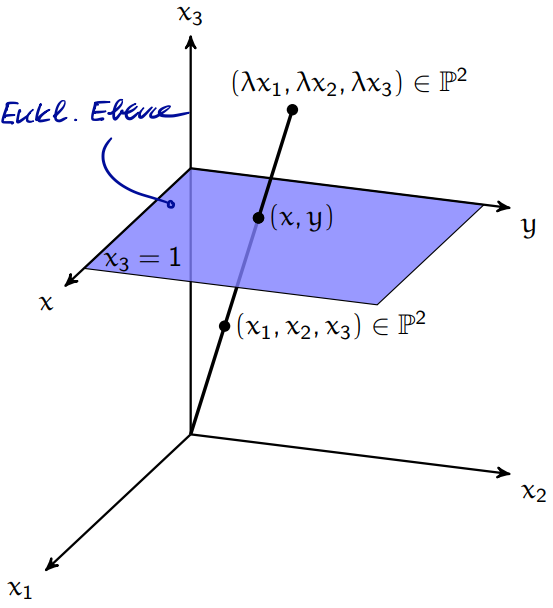
\includegraphics[width=0.24\textwidth]{assets/euclidean-plane.png}
    }
    & \textit{Ein Punkt auf der euklid-} \\
    & \textit{ischen Ebene entspricht} \\
    & \textit{dem Wert eines dehomogen-} \\
    & \textit{isierten Punktes $(x,y)$.} \\
    & \\
    & \textit{$x_3 = 1$ ergibt die} \\
    & \textit{euklidische Ebene.} \\
    & \\
    & \textit{$\lambda(x_1, x_2, x_3)$ sind Punkte} \\
    & \textit{auf einer Gerade die den Punkt} \\
    & \textit{$(\frac{x_1 \lambda}{x_3 \lambda}, \frac{x_2 \lambda}{x_3 \lambda}) = (x,y)$ definieren.} \\
\end{tabular} \\

\subsection{Projektive Transformation}

\textit{
    Abbildungen $h: \mathbb{P}^2 \mapsto \mathbb{P}^2$
    mit Eigenschaften:
}

\begin{itemize}
    \item $h$ ist eindeutig (bijektiv) und daher umkehrbar
    \item $h$ Transformationen sind geradentreu (geraden auf geraden abbilden)
    \item \textbf{Homogene Matrix} ist bis auf eine Konstante bestimmt ($k\mathbf{H} = \mathbf{H}$; $k > 0$)
\end{itemize}

$\vec{r}' = h(\vec{r}) = \mathbf{H} \vec{r}$, $\mathbf{H} = \begin{bmatrix}
    h_{11} & h_{12} & h_{13} \\
    h_{21} & h_{22} & h_{23} \\
    h_{31} & h_{32} & h_{33} \\
\end{bmatrix}$

\subsection{Transformationen kombinieren}

$\vec{r} ' = h(\vec{r}) = (h_2 \circ h_1)(\vec{r}) = h_2(h_1(\vec{r}))$\\

$\mathbf{H} = \mathbf{H}_2\mathbf{H}_1$,
$\vec{r} ' = \mathbf{H}\vec{r} = \mathbf{H}_2 \cdot \mathbf{H}_1\vec{r}$

\textit{\\
    $h_1: \mathbb{P}^2 \mapsto \mathbb{P}^2$,
    $h_2: \mathbb{P}^2 \mapsto \mathbb{P}^2$ \\
    $h = h_2 \circ h_1$ entspricht erst $h_2$ dann $h_1$
}

\subsection{Translation 2D}

$\vec{r} ' = \left[\begin{array}{cc|c}
    1 & 0 & t_x \\
    0 & 1 & t_y \\
    \hline
    0 & 0 & 1 \\
\end{array}\right]
\vec{r} = \mathbf{T} \vec{r}$ \\

\textit{Verschiebung durch $\vec{t} = \begin{bmatrix}
    t_x \\
    t_y \\
\end{bmatrix}$, $\mathbf{T}^{-1}$ entspricht $-\vec{t}$ in $\mathbf{T}$}

\subsection{Nullpunkt Rotation 2D}

$\vec{r}' = \left[\begin{array}{cc|c}
    \cos(\phi) & -\sin(\phi) & 0 \\
    \sin(\phi) & \cos(\phi) & 0 \\
    \hline
    0 & 0 & 1 \\
\end{array}\right] = \mathbf{R} \vec{r}$

\textit{Rotation mit $\phi$, $\mathbf{R}^{-1}$
entspricht $\sin$ vertauschen}

\subsection{Rotation um Punkt $A$}

\textit{Punkt: $A(t_x, t_y)$}

\begin{enumerate}
    \item Translation $A$ zum Nullpunkt verschiebt ($\mathbf{T}$)
    \item Nullpunkt Rotation 2D mit Winkel $\Phi$
    \item Translation $A$ zurück ($\mathbf{T}^{-1}$)
\end{enumerate}

$\mathbf{R} = \mathbf{T}^{-1} \mathbf{R}_0 \mathbf{T} = \begin{bmatrix}
    1 & 0 & t_x \\
    0 & 1 & t_y \\
    0 & 0 & 1 \\
\end{bmatrix} \begin{bmatrix}
    \cos(\Phi) & -\sin(\Phi) & 0 \\
    \sin(\Phi) & \cos(\Phi) & 0 \\
    0 & 0 & 1 \\
\end{bmatrix} \begin{bmatrix}
    1 & 0 & -t_x \\
    0 & 1 & -t_y \\
    0 & 0 & 1 \\
\end{bmatrix}$

\subsection{Spiegelung mit Gerade durch Ursprung}

\begin{tabular}{cl}
    \multirow{8}{*}{
        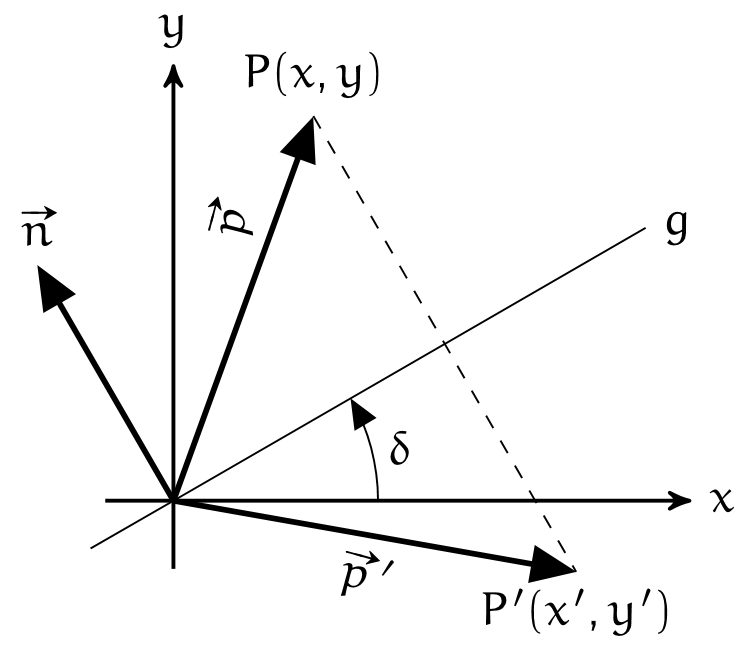
\includegraphics[width=0.2\textwidth]{assets/mirror-on-line.png}
    } & $\vec{n} = (-\sin(\delta), cos(\delta))^T$ \\
    & \\
    & HNF: $-\sin(\delta)x + cos(\delta)y = 0$\\
    & \\
    & $\vec{p}' = \vec{p} - 2 (\vec{p} \bullet \vec{n}) \vec{n}$\\
    & \\
    & $\delta = \arctan(\frac{y}{x})$ \\
    & \textit{Wenn $g$ geht durch Nullpunkt}\\
\end{tabular}

$\vec{r}' = \left[\begin{array}{cc|c}
    \cos(2\delta) & \sin(2\delta) & 0 \\
    \sin(2\delta) & -\cos(2\delta) & 0 \\
    \hline
    0 & 0 & 1 \\
\end{array}\right] \vec{r}$

\subsection{Spiegelung mit Gerade $g$}

\begin{enumerate}
    \item gerade ins Zentrum Transformieren ($\mathbf{T}$ errechnen)
    \item Spiegelung mit Gerade durch Ursprung ($\mathbf{S}$)
    \item zurück Transformieren ($\mathbf{T}^{-1}$)
\end{enumerate}

$\mathbf{M} = \mathbf{T^{-1}ST}$

\subsection{Transformation des Koordinatensystemes}

$ \begin{bmatrix}
    \cos(-\Phi) & -\sin(-\Phi) & 0 \\
    \sin(-\Phi) & \cos(-\Phi) & 0 \\
    0 & 0 & 1 \\
\end{bmatrix}$

\textit{Rotation des Koordinatensystemes um $\Phi$}

\textit{Bei einer Transformation des Koordinatensystemes
handelt es sich um eine Inverse Matrix der normalen
Transformation}

\subsection{Transformationen 2D}

$t=\begin{bmatrix}
    x \\
    y \\
\end{bmatrix}$, $0^T = \begin{bmatrix}
    0 \\
    0 \\
\end{bmatrix}$, $\mathbf{RMC} =$ 2x2 Matrix

\textbf{Euklidisch} (starre Bewegung) \\
$D = \begin{bmatrix}
    \mathbf{R} & t \\
    0^T & 1
\end{bmatrix}$ \\
\textit{Abstand zwischen zwei Punkten, alle Winkel} \\
\textit{($R^{-1} = R^T$)} \\

\textbf{Ähnlichkeit} \\
$S = \begin{bmatrix}
    k \cdot \mathbf{M} & t \\
    0^T & 1
\end{bmatrix}$ \\
\textit{Winkel zwischen zwei Punkten, alle Winkel} \\

\textbf{Affin} \\
$A = \begin{bmatrix}
    \mathbf{C} & t \\
    0^T & 1
\end{bmatrix}$ \\
\textit{Parallelität, Verhältnis zwischen Flächeninhalte} \\

\textbf{Allgemein} \\
$\mathbf{H} = \begin{bmatrix}
    h_{11} & h_{12} & h_{13} \\
    h_{21} & h_{22} & h_{23} \\
    h_{31} & h_{32} & h_{33} \\
\end{bmatrix}$ \\
\textit{Geraden bleiben Geraden} \\

\section{Transformation}

\subsection{Transformation des Koordinatenystems}

TODO

\subsection{homogene Koordinaten}

\textit{jeder Punkt P(x,y,z) des Raumes $\mathbb{R^3}$ besitzt eine 4-komponenten Vektor $\vec{r}$}
\\
$\vec{r} = \begin{bmatrix}
    x_1 \\
    x_2 \\
    x_3 \\
    x_4
\end{bmatrix}$, 
$x = \frac{x_1}{x_4}$, 
$y = \frac{x_2}{x_4}$, 
$z = \frac{x_3}{x_4}$ \\

$(x,y,z) = (\frac{x_1}{x_4}, \frac{x_2}{x_4}, \frac{x_3}{x_4})$

\subsection{Ebene im Raum}

\textit{Ebene $\epsilon$ im Raum $\mathbb{R}^3$}
\\
$\epsilon : ax + by + cz + d = 0$
\textit{Hessische Normalform}
\\ \\
$\vec{w} = \begin{bmatrix}
    a \\
    b \\
    c \\
    d
\end{bmatrix}$, Punkt:
$\vec{r} = \begin{bmatrix}
    x \\
    y \\
    z \\
    1
\end{bmatrix}$ \\

\textit{Ebenengleichung:}

$\vec{w} \bullet \vec{r} = w^T \cdot r = ax + by + cz + d = 0$ \\

\subsection{Prokektive Transformation}

\textit{Die homogene Matrix $\mathbf{H}$ ist nur bis auf einen konstanten \
 Faktor bestimmt, heisst, alle Vielfachen von $\mathbf{H}$ sind auch gültig} \\

\text{$\eta : \mathbb{P}^3 \mapsto \mathbb{P}^3 $ stellt eine \textbf{projektiven Transformation} dar} \\

$\eta(r) = \mathbf{H} \cdot r = \begin{bmatrix}
    h_{11} & h_{12} & h_{13} & h_{14} \\
    h_{21} & h_{22} & h_{23} & h_{24} \\
    h_{31} & h_{32} & h_{33} & h_{34} \\
    h_{41} & h_{42} & h_{43} & h_{44}
\end{bmatrix} \cdot \begin{bmatrix}
    x_1 \\
    x_2 \\
    x_3 \\
    x_4 
\end{bmatrix}$

\textbf{Euklidisch} (starre Bewegung) \\
$D = \begin{bmatrix}
    \mathbf{R} & t \\
    0^T & 1
\end{bmatrix}$ \\
\textit{Abstand zwischen zwei Punkten, alle Winkel} \\
\textit{($R^{-1} = R^T$)} \\

\textbf{Ähnlichkeit} \\
$S = \begin{bmatrix}
    k \cdot \mathbf{M} & t \\
    0^T & 1
\end{bmatrix}$ \\
\textit{Winkel zwischen zwei Punkten, alle Winkel} \\

\textbf{Affin} \\
$A = \begin{bmatrix}
    \mathbf{C} & t \\
    0^T & 1
\end{bmatrix}$ \\
\textit{Parallelität, Verhältnis zwischen Volumeninhalt} \\

\textbf{Allgemein} \\
$\mathbf{H} = \begin{bmatrix}
    h_{11} & h_{12} & h_{13} & h_{14} \\
    h_{21} & h_{22} & h_{23} & h_{24} \\
    h_{31} & h_{32} & h_{33} & h_{34} \\
    h_{41} & h_{42} & h_{43} & h_{44}
\end{bmatrix}$ \\
\textit{Geraden bleiben Geraden} \\

\subsection{Euklidische Transformationen}

TODO Translation, Spiegelung an einer Ebene, Rotation, Zusammensetzen von

\subsection{Rotation um beliebige Achse}

1) Rotation um $\phi$ um z-Achse (Matrix D) \\
2) Rotation um den Winkel $\theta \in [0, \pi]$ (um frühere X-Achse) (Matrix C)  \\
3) Eigentlich Rotation um den gegeben Winkel $\psi$ (Matrix B) \\

\textit{$c_\alpha = \cos \alpha$, $s_\alpha = \cos \alpha$, $\alpha \in {\phi, \theta, \psi}$} \\

\newcolumntype{C}{>{\centering\arraybackslash} m{6cm} }
\begin{tabular}{m{3cm}CC}
    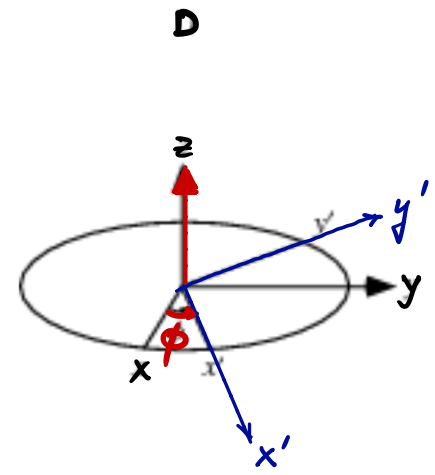
\includegraphics[scale=0.3]{rotation_matrix_D} &
    $\mathbf{D} = \begin{bmatrix}
        c_\phi & s_\phi & 0 \\
        -s_\phi & c_\phi & 0 \\
        0 & 0 & 1 
    \end{bmatrix}$ \\
\end{tabular} \\
\begin{tabular}{m{3cm}CC}
    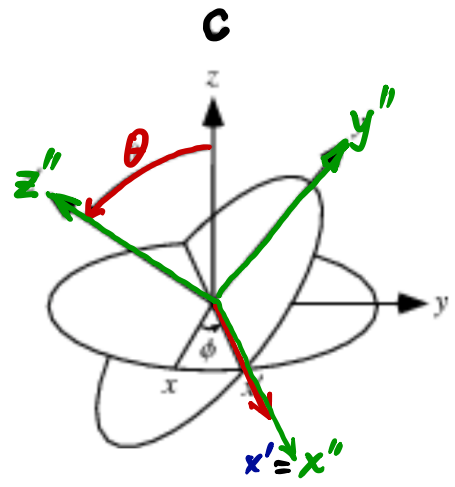
\includegraphics[scale=0.3]{rotation_matrix_C} &
    $\mathbf{D} = \begin{bmatrix}
        1 & 0 & 0 \\
        0 & c_\theta & s_\theta \\
        0 & -s_\theta & c_\theta
    \end{bmatrix}$ \\
\end{tabular} \\
\begin{tabular}{m{3cm}CC}
    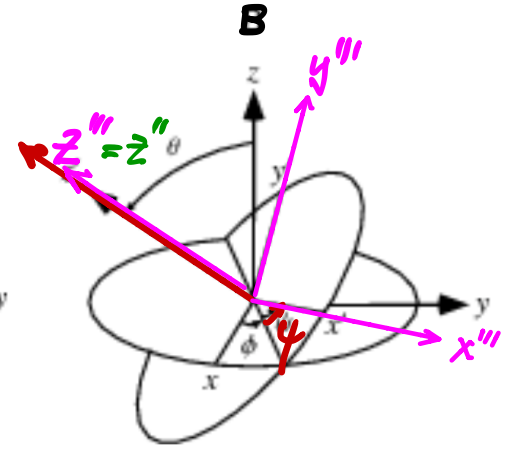
\includegraphics[scale=0.3]{rotation_matrix_B} &
    $\mathbf{D} = \begin{bmatrix}
        c_\psi & s_\psi & 0 \\
        -s_\psi & c_\psi & 0 \\
        0 & 0 & 1
    \end{bmatrix}$ \\
\end{tabular}

Danach wieder zurück rotieren um $\phi$ und $\theta$

\subsection{Rotation um eine Achse durch den Ursprung}

TODO insert T / $R_{y,x,z}$ \\

Todo rotation around any axis \\

Todo altertative, rotation around origin \\

\subsection{Parallele Projektion}

\textit{Projektion auf Ebene $\epsilon: ax + by + cz + d = 0$} \\
\textit{Die ebene ist definiert durch Normalvektor $\vec{n} = \begin{bmatrix}
    a \\
    b \\
    c
\end{bmatrix}$} \\
\textit{Normalenvektor erhalten: $|\vec{n}| = \sqrt{a^2 + b^2 + c^2} = 1$} \\

\textit{Projektionsrichtung definiert durch $\vec{v} = (v_x, v_y, v_z)$} \\
\textit{Normalisieren von Projektionsrichtung: $|\vec{v}|$} \\

\textit{Ist $|\vec{n}|$ (Ebenen Normalenvektor) und $|\vec{v}|$ (Projektionsrichtung) gegeben} \\

$\vec{x} = \vec{x}_0 + t\vec{v}$, komponentenweise $\begin{bmatrix}
    x = x_0 + tv_x \\
    y = y_0 + tv_y \\
    y = y_0 + tv_y
\end{bmatrix}$ \\
\textit{Wobei $x_0$ Punkt wo auf $x$ auf Ebene Projeziert wird} \\

\textit{$\psi$ entspricht Winkel zwischen $\vec{n}$ und $\vec{v}$} \\

$cos(\psi) = \vec{v} \bullet \vec{n}$

TODO - gleichung t t* \\

\subsection{Parallele Projektionsmatrix}

$\begin{bmatrix}
    x^* \\
    y^* \\
    z^*
\end{bmatrix} = \mathbf{H} \begin{bmatrix}
    x_0 \\
    y_0 \\
    z_0
\end{bmatrix} = $ \\
$\frac{1}{c_\psi} \begin{bmatrix}
    (c_\psi - av_x) & -bv_x & -cv_x & -dv_x \\
    -av_y & (c_\psi - bv_y) & -cv_y & -dv_y \\
    -av_z & -bv_z & (c_\psi - cv_z) & -dv_z \\
    0 & 0 & 0 & c_\psi
\end{bmatrix} \begin{bmatrix}
    x_0 \\
    y_0 \\
    z_0 \\
    1
\end{bmatrix}$ \\
\textit{$cos(\psi) = c_\psi$}

\subsection{Perspektivische Projektion}

\textit{Fall wenn Zentrum $O$ im Nullpunkt} \\

$\epsilon: ax + by + cz + d = 0$, Ebene \\

\textit{Beliebigen Punkt $A_0(x_0,y_0,z_0)$ mit Projektionspunkt $A^*(x^*,y^*,z*)$ in Ebene $\epsilon$} \\

$\begin{bmatrix}
    x^* \\
    y^* \\
    z^* \\
\end{bmatrix} = \begin{bmatrix}
    \lambda x_0 \\
    \lambda y_0 \\
    \lambda z_0 
\end{bmatrix}$ \\

$\lambda = - \frac{d}{ax_0 + by_0 + cz_0}$ \\

$(ax_0 + by_0 + cz_0) \cdot \begin{bmatrix}
    x^* \\
    y^* \\
    z^* \\
    1
\end{bmatrix} = \begin{bmatrix}
    -dx_0 \\
    -dy_0 \\
    -dz_0 \\
    ax_0 + by_0 + cz_0
\end{bmatrix} = \begin{bmatrix}
    -d & 0 & 0 & 0 \\
    0 & -d & 0 & 0 \\
    0 & 0 & -d & 0 \\
    a & b & c & 0
\end{bmatrix} \begin{bmatrix}
    x_0 \\
    y_0 \\
    z_0 \\
    1
\end{bmatrix}$ \\

\subsection{Perspektivische Projektionmatrix}

$\mathbf{H} = \begin{bmatrix}
    -d & 0 & 0 & 0 \\
    0 & -d & 0 & 0 \\
    0 & 0 & -d & 0 \\
    a & b & c & 0
\end{bmatrix}$ \\

\subsection{Sichtvolumen Clipping}

\textit{Das kanonische Sichtvolmen ist ein Würfel mit $P(\pm 1, \pm 1, \pm 1)$} \\
\textit{Defür sind vorne und hinten, sowie zwei Punkte bestimmend Grösse gegeben} \\

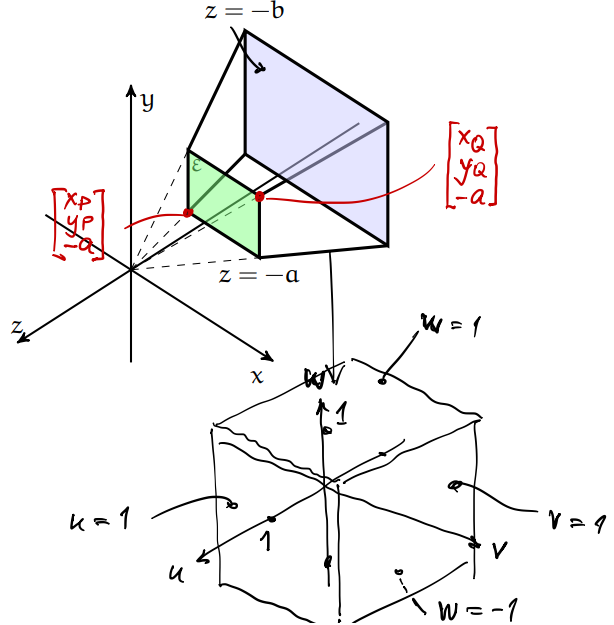
\includegraphics[scale=0.4]{clipping} \\

\textit{$P$ links unten, $Q$ rechts oben} \\
\textit{$z$ vorne $z=-a$, $z$ hinten $z=-b$} \\

$\mathbf{T} = \begin{bmatrix}
    \frac{2a}{x_Q - x_P} & 0 & \frac{x_Q + x_P}{x_Q - x_P} & 0 \\
    0 & \frac{2a}{y_Q - y_P} & \frac{y_Q + y_P}{y_Q - y_P} & 0 \\
    0 & 0 & -\frac{b+a}{b-a} & -2\frac{ba}{b-a} \\
    0 & 0 & -1 & 0 \\
\end{bmatrix}$


\section{Scan Konvertierung}

\subsection{Linie Rastern}

\textit{Eine Linie von $(x_0, y_0)$ nach $(x_1, y_1)$ rastern. Da in Pixel konvertiert werden muss. Methoden:}

\begin{itemize}
    \item \textit{Brute Force; über jeden Pixel und runden}
    \item \textit{Brute Force inkrementell (DDA = Digital Differential Analyzer); $y_{i+1} = m * x_{i+1) + B = y_i + m}$,
          Nachteil Gleitkommazahlen und Runden (aufwändig)}
    \item \textit{Mittelpunktschema; Nächsten Punkt wird Kalkuliert durch if / else}
\end{itemize}

\subsection{Mittelpunktschema}
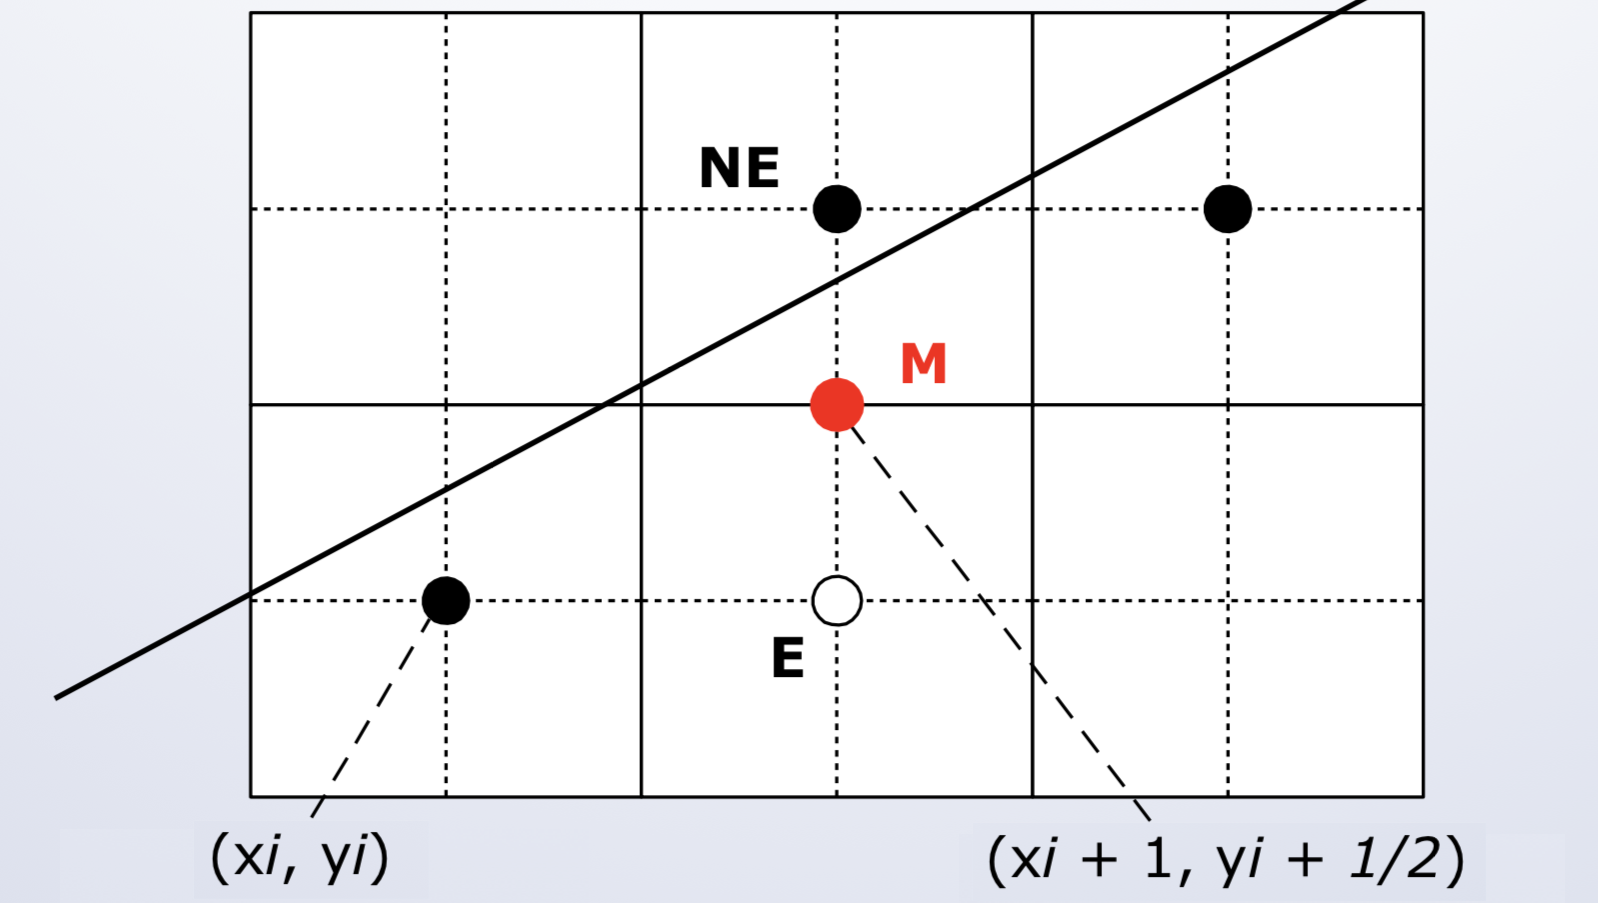
\includegraphics[width=0.35\textwidth]{assets/Mittelpunktschema.png}

\textit{Ist eine inkrementelle methode zum Rastern. Mittelpunkt
wird betrachtet um nächsten Punkt zu finden. ($M = (x_i+1, y_i+\frac{1}{2})$, $E = (x_i+1, y_i)$, $NE = (x_i+1, y_i+1)$)}\\

Initialisierung:\\
$D_x = x_1 - x_0$; \\
$D_y = y_1 - y_0$; \\
$D_E = 2 * D_y$; \\
$D_{NE} = 2 * (D_y - D_x)$; \\
$d = 2*D_y - D_x$; \\
$y = y_0$ \\

\textit{Wegen 1/2 alles mal 2, damit gerade Zahlen}

\textit{
    Für jeden nächsten $d$ Wert, wenn $d <= 0$,
    dann $d = d + D_{NE}$ ansonsten $d = d + D_{NE}$ und $y$ inkremenrieren.
    Jeweils den Punkt $P(x,y)$ zeichnen. $x$ jedesmal inkrementieren.
}

Berechnung:
\begin{lstlisting}
WritePixel(x0, y0)
for x = x0+1 to x1 do
  if d <= 0 then
    d = d + DE;
  else
    d = d + DNE;
    y = y + 1;
  end
  WritePixel(x,y);
end
\end{lstlisting}

\subsection{Kreis Rastern}

\textit{Selbe Methode wie bei den Linien kann für Kreise angewendet werden.}

\subsection{Mittelpunktschema Kreis}

\textit{Funktion für Kreis: $F(x,y) = x^2 + y^2 - R^2$}\\

$x = 0$\\
$y = R$\\
$d = 1 - R$\\
$D_{E} = 2*x + 3$\\
$D_{NE} = 2*(x-y)d + 5$\\

\textit{
    Für jeden nächsten $d$ Wert wiederholen bis $y > x$, wenn $d < 0$,
    dann $d = d + D_{E}$ ansonsten $d = d + D_{NE}$ und $y$ dekrementieren.
    Jeweils den Punkt $P(x,y)$ zeichnen. $x$ jedesmal inkrementieren.
}

\begin{lstlisting}
WritePixel(x,y);
while y > x do
  if d < 0 then
    d = d + 2*x + 3;
  else
    d = d +2*(x-y) + 5;
    y = y - 1;
  end
  x = x + 1;
  WritePixel(x,y);
end
\end{lstlisting}

\subsection{Regionen füllen}

\textit{Entweder durch 4-er oder 8-er Zusammenhang definiert}

\begin{tabular}{cl}
    \multirow{3}{*}{
        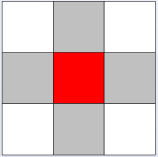
\includegraphics[width=0.05\textwidth]{assets/region-filling-4.png}
    } & \\
    & \textit{4-er Zusammenhang} \\
    & \\
\end{tabular}
\begin{tabular}{cl}
    \multirow{3}{*}{
        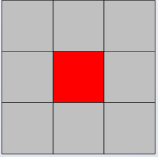
\includegraphics[width=0.05\textwidth]{assets/region-filling-8.png}
    } & \\
    & \textit{8-er Zusammenhang} \\
    & \\
\end{tabular}

\subsubsection{FloodFill}

\textit{Füllen durch selben abfrage ob selbe Farbe (Photoshop Zauberstab)}
\begin{lstlisting}
proc FloodFill(int x, int y,
Color oldColor, Color newColor)
  if ReadPixel(x,y) == oldColor then
    WritePixel(x,y,newColor);
    FloodFill(x, y-1, oldColor, newColor);
    FloodFill(x-1,y, oldColor, newColor);
    FloodFill(x, y+1, oldColor, newColor);
    FloodFill(x+1, y, oldColor, newColor);
  end
end
\end{lstlisting}

\subsection{Zeichnen von gefüllten Polygonen}

\subsubsection{Scanlinien Algorithmus}

\begin{tabular}{cc}
  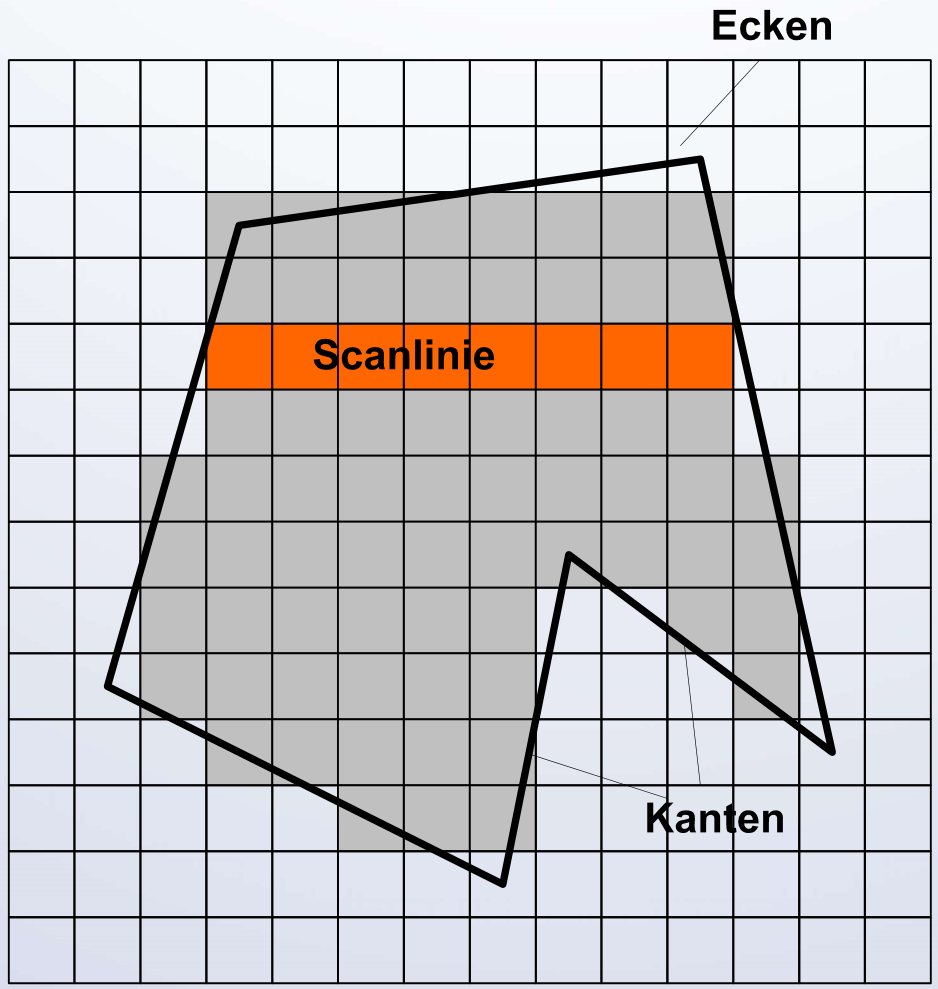
\includegraphics[width=0.25\textwidth]{assets/scanlinien-alg.png} &
  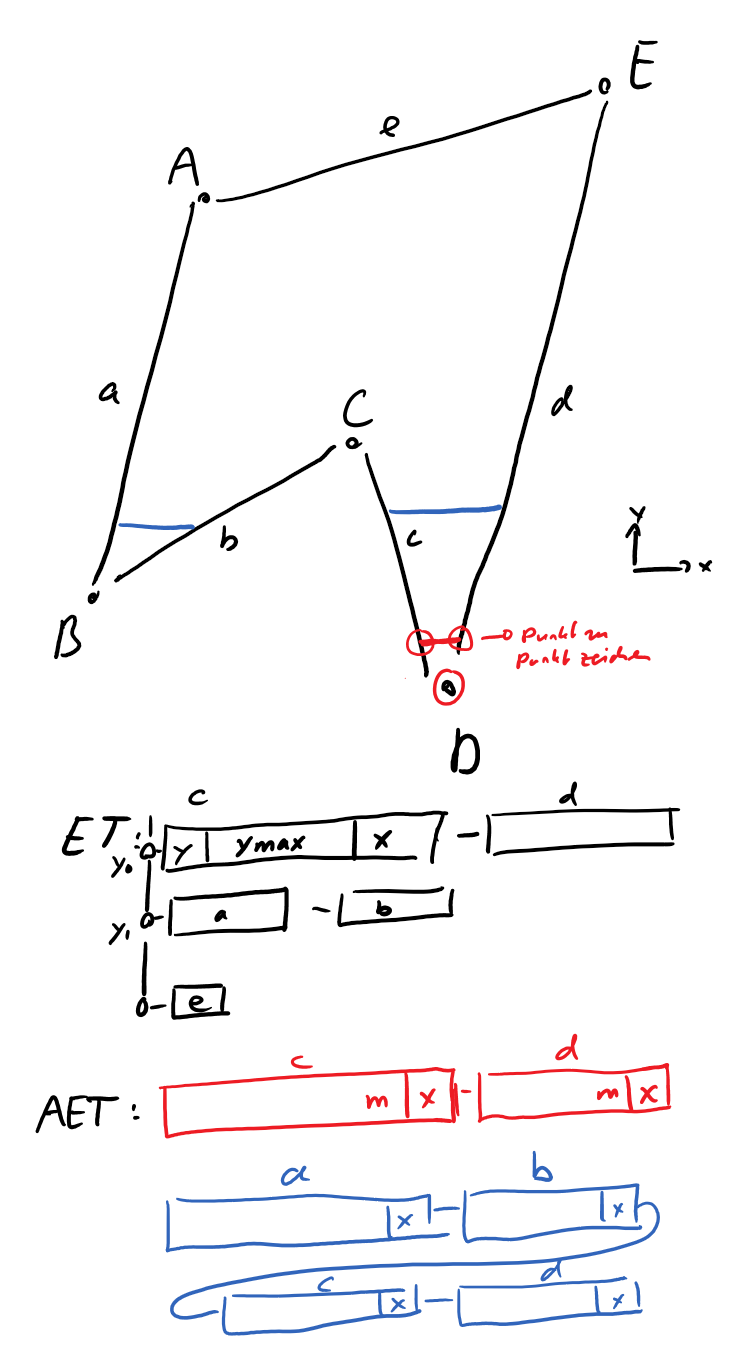
\includegraphics[width=0.25\textwidth]{assets/scanlinien-alg-demo.png} \\
\end{tabular}

\begin{itemize}
	\item Zeilenweise färben (Spans entlang der y Koordinate -> Scanlinien)
	\item Kantentabelle (edgetable ET)\\
    sortierte Kanten (Linien) des Polygon nach min y (innerhalb davon nach max x)
  \item Einträge werden gespeichert durch $[x|l/m|y_{min}|y_{max}]$
	\item Tabelle aktiver Kanten (AET)\\
		Momentane Kanten für Scanlinie (sortiert nach x asc) zum Zeichnen vom einer Kante zur nächsten (immer zwei)
\end{itemize}

\begin{lstlisting}
Erzeuge ET (Kantentabelle)
Initialisiere AET = empty  (Aktive Kanten)
y=0
repeat
  Addiere und entferne alle Kanten
      ET(y) zu AET
  Sortiere AET nach x
  Zeichne Spans
  y=y+1
  Entferne Kanten mit ymax = y aus AET
  Aktualisiere den x Wert aller
      Kanten in AET
until AET == empty and ET == empty
\end{lstlisting}

\subsubsection{Zeichnen von Dreiecken}

\textit{Brute Force: Alle Pixel probieren, ob im Dreieck}

\begin{tabular}{cl}
  \multirow{3}{*}{
      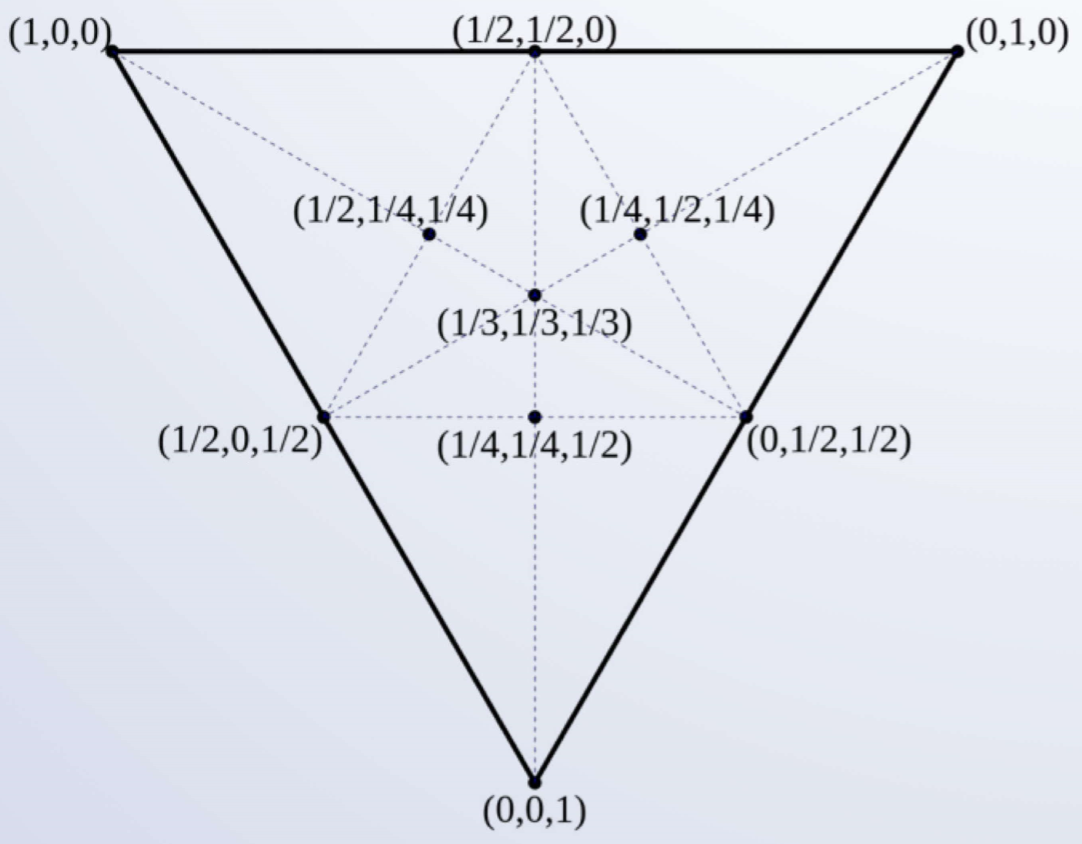
\includegraphics[width=0.2\textwidth]{assets/draw-baryzentrische-coordinates.png}
  } & \\
  & Baryzentrische Koordinaten \\
  & \\
  & $P = \alpha A + \beta B + \gamma C$\\
  & \\
  & $\alpha+\beta+\gamma =1$\\
  & \\
\end{tabular}

\textit{Wenn Werte zwischen 0 und 1, dann ist Punkt P innerhalb von ABC.
Wert einer Koordinate entspricht dem Verhältnis der Fläche eines Teildreiecks
mit Ecke P zur Fläche von ABC}\\

\begin{tabular}{cl}
  \multirow{3}{*}{
    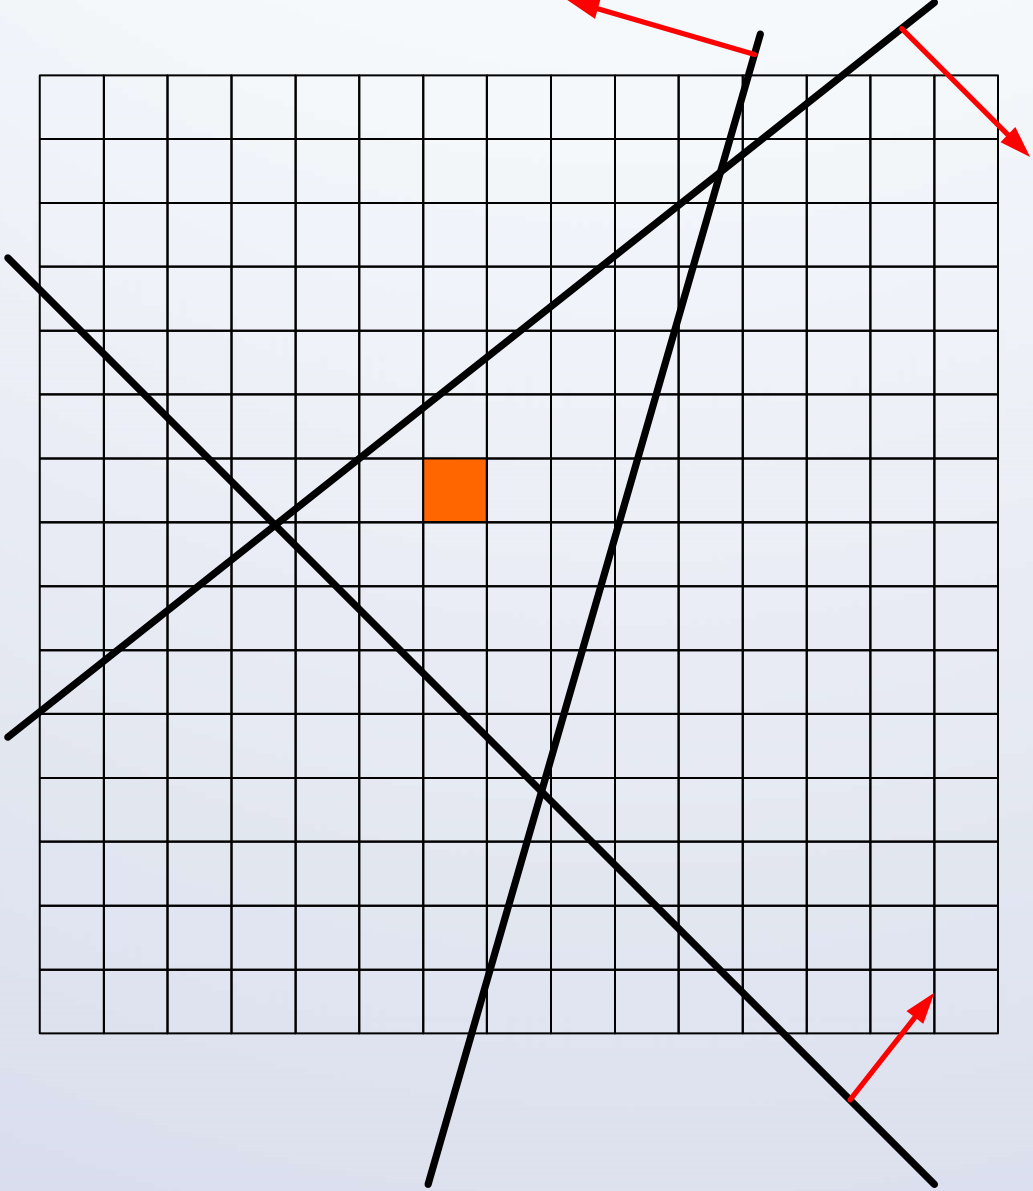
\includegraphics[width=0.15\textwidth]{assets/draw-line-side.png}
  } & 2. Bruteforce Option \\
  & \\
  & Unterteilung in 3 Geraden. \\
  & Zeichnen wenn auf der richtigen\\
  & Seite aller Geraden \\
  & \\
  & \\
\end{tabular}

\subsection{Anti-Aliasing}
\textit{Treppenmuster vermeiden}
\begin{itemize}
	\item Prefiltering -> Farbintensität proportional zur Fläche oder Linie
  \item Supersampling -> Bild mit höherer Auflösung berechnen und Farbmittelwerte
    als Übergänge zeichnen (4x Sample Patter, Quincunx AA Sample Pattern)
\end{itemize}


\section{Curves}

\subsection{Kurvie in der Ebene}

\textbf{Explizite Darstellung} \\
$\gamma : [a,b] \rightarrow \mathbb{R} , x \mapsto y = f(x)$ \\
\textit{Kreis: \\oberer Halbkreis $\sqrt{r^2 - x^2}$ \\ unterer Halbkreis $\sqrt{r^2 - x^2}$} \\
\\
\textbf{Implizite Darstellung} \\
$F(x,y) = 0$ \\
\textit{Kreis: $x^2 + y^2 - r^2 = 0$} \\
\\
\textbf{Parameterdarstellung} \\
$\gamma : [a,b] \rightarrow \mathbb{R}^2,t \mapsto X(t) = \begin{bmatrix} x_1(t) \\ x_2(t) \end{bmatrix}$ \\
\textit{Punkte miteinander verbunden, einzeln angegeben} \\
\textit{Kreis: $\begin{bmatrix} r \cos t \\ r \sin t \end{bmatrix}$}
\\

\subsection{Kurve im Raum}

$\gamma : [a,b] \rightarrow \mathbb{R}^3,t \mapsto X(t) = 
\begin{bmatrix}
    x_1(t) \\
    x_2(t) \\
    x_3(t)
\end{bmatrix}$

\subsection{Spirale entlang des Zylinders}

$x^2 + y^2 = r^2$ \\
$\gamma : [0, 4\pi] \rightarrow \mathbb{R}^3, t \mapsto X(t) = \begin{bmatrix}
    r \cos t \\ r sin t \\ ht / (2\pi)
\end{bmatrix}$ \\
\textit{Grundriss ergibt Kreis, Höhe Linear}

\subsection{Methode unbestimmte Koeffizienten}

$P_3(x) = c_0 + c_1x^2 + c_2x^2 + c_3x^3$ \\
\\
$\begin{bmatrix}
    1 & x_0 & x_0^2 & x_0^3 \\
    1 & x_1 & x_1^2 & x_1^3 \\
    1 & x_2 & x_2^2 & x_2^3 \\
    1 & x_3 & x_3^2 & x_3^3 \\
\end{bmatrix} 
\begin{bmatrix}
    c_0 \\
    c_1 \\
    c_2 \\
    c_3
\end{bmatrix} = 
\begin{bmatrix}
    y_0 \\
    y_1 \\
    y_2 \\
    y_3
\end{bmatrix}$ \\
\\
\textit{$c_0 = c_1 = c_2 = c_3 = 1$}

\subsection{Lagrange Methode}

$l_0(x) = (x-x_1)(x-x_2)\dots$ \\
$L_0(x) = \frac{l_0(x)}{l_0(x_0)} = \frac{(x-x_1)(x-x_2)\dots}{(x_0-x_1)(x_0-x_2)\dots}$ \\
$P_n(x) = y_0L_0(x)+y_1L_1(x)+ \dots + y_nL_n()$ \\
\\
$l_k(x) = \prod^{n}_{i=0 \\ i \neq k}(x-x_i)$ \\
$L_k(x) = \frac{l_k(x)}{l_k(x_k)}$

\subsection{Lineare Bézier spline}

$P(t) = (1 - t) P_0 + P_1 (0 \leq t \leq 1)$ \\
\textit{Gewichteter Durchschnitt der Kontrollpunkte} \\
\\
$P(t) = (P_1 - P_0) t + P_0$ \\
\textit{Polynom in $t$} \\
\\
$P(t) = [P_0, P_1] \begin{bmatrix}
    -1 & 1 \\ 1 & 0
\end{bmatrix}
\begin{bmatrix}
    t \\ 1
\end{bmatrix} (0 \leq t \leq 1)$ \\
\textit{Matrizform}

\subsection{Quadric Bézier spline}

\textit{drei Kontrollpunkte $P_0, P_1, P_2$}\\

$P_0^1(t) = (1-t)P_0 + P_1$ \\
$P_1^1(t) = (1-t)P_0 + P_1$ \\

$P(t) = (1 - t)^2P_0 + 2(1 - t)tP_1 + t^2 P_2$

\subsection{Qubic Bézier Spline}

\textit{vier Kontrollpunkte $P_0, P_1, P_2, P_3$}\\

\textit{Mit $P_0^1$, $P_1^1$ und} \\
$P_2^1(t) = (1-t)P_2 + tP_3$ \\

$P_1^2(t) = (1 - t) P_0^1(t) + tP_1^1(t)$ \\
$P_2^2(t) = (1 - t) P_1^1(t) + tP_2^1(t)$ \\

$P(t) = (1 - t)^3P_0 + 3(1 - t)^2tP_1 + 3(1 - t)t^2P_2 + t^3P_3$

\subsection{Bernsteinpolynome}




\section{Appendix}

\subsection{Radians}

\begin{tabular}{cccc}
    Winkel $\alpha^\circ$ & Bogenmass & Sinus & Kosinus \\ [1.5ex] \hline
    $0^\circ$ & $0$ & $\frac{1}{2}\sqrt{0} = 0$ & $\frac{1}{2}\sqrt{4} = 1$ \\ [1.5ex] \hline
    $30^\circ$ & $\frac{\pi}{6}$ & $\frac{1}{2} \sqrt{1} = \frac{1}{2}$ & $\frac{1}{2} \sqrt{3}$ \\ [1.5ex] \hline
    $45^\circ$ & $\frac{\pi}{4}$ & $\frac{1}{2}\sqrt{2} = \frac{1}{\sqrt{2}}$ & $\frac{1}{2}\sqrt{2} = \frac{1}{\sqrt{2}}$ \\ [1.5ex] \hline
    $60^\circ$ & $\frac{\pi}{3}$ & $\frac{1}{2}\sqrt{3}$ & $\frac{1}{2}\sqrt{1} = \frac{1}{2}$ \\ [1.5ex] \hline
    $90^\circ$ & $\frac{\pi}{2}$ & $\frac{1}{2}\sqrt{4} = 1$ & $\frac{1}{2} \sqrt{0} = 0$ \\ [1.5ex] \hline
    $180^\circ$ & $\pi$ & $0$ & $-1$ \\ [1.5ex] \hline
    $270^\circ$ & $\frac{3\pi}{2}$ & $-1$ & $0$ \\ [1.5ex] \hline
    $360^\circ$ & $2\pi$ & $0$ & $1$ \\ [1.5ex] \hline
\end{tabular} \\
\\
$\cos^2(\alpha) = \frac{1}{1 + \tan^2(\alpha)}$ \\
$\sin^2(\alpha) = \frac{\tan^2(\alpha)}{1 + \tan^2(\alpha)}$ \\
$\sin(\alpha + \beta) = \sin \alpha \cos \beta + \cos \alpha \sin \beta$ \\
$\cos(\alpha + \beta) = \cos \alpha \cos \beta - \sin \alpha \sin \beta$ \\
$\cos(\alpha) = \cos(-\alpha)$ \\
$\sin(-\alpha) = -\sin(\alpha)$ \\


\end{document}
